%%%%%%%%%%%%%%%%%%%%%%%%%%%%%%%%%%%%%%%%%%%%%%%%%%%%%%%%%%%%%%%%%%%%%
% LaTeX Template: Project Titlepage Modified (v 0.1) by rcx
%
% Original Source: http://www.howtotex.com
% Date: February 2014
%
% This is a title page template which be used for articles & reports.
%
% This is the modified version of the original Latex template from
% aforementioned website.
%
%%%%%%%%%%%%%%%%%%%%%%%%%%%%%%%%%%%%%%%%%%%%%%%%%%%%%%%%%%%%%%%%%%%%%%

\documentclass[12pt]{report}
\usepackage[a4paper]{geometry}
\usepackage[myheadings]{fullpage}
\usepackage{fancyhdr}
\usepackage{lastpage}
\usepackage{graphicx, wrapfig, subcaption, setspace}
\graphicspath{ {img/} }
\usepackage[T1]{fontenc}
\usepackage[font=small, labelfont=bf]{caption}
\usepackage{fourier}
\usepackage[protrusion=true, expansion=true]{microtype}
\usepackage[english]{babel}
\usepackage{sectsty}
\usepackage{url, lipsum}
\usepackage{amsmath}
\usepackage{xfrac}
\usepackage{pgfgantt}
\usepackage{lscape}
\usepackage{url}
\usepackage{bm}
\usepackage{listings}
\usepackage{tabularx}
\usepackage[utf8]{inputenc}

\setlength{\parindent}{0em}
\setlength{\parskip}{1.2em}

\newcommand{\HRule}[1]{\rule{\linewidth}{#1}}
\onehalfspacing

%-------------------------------------------------------------------------------
% HEADER & FOOTER
%-------------------------------------------------------------------------------
\pagestyle{fancy}
\fancyhf{}
\setlength\headheight{15pt}
\fancyhead[L]{Similar nodes in large graphs}
\fancyhead[R]{Vlad Velici}
\fancyfoot[R]{Page \thepage\ of \pageref{LastPage}}
%-------------------------------------------------------------------------------
% TITLE PAGE
%-------------------------------------------------------------------------------

%% USEFUL DEFINITIONS

\setcounter{secnumdepth}{2}
\setcounter{tocdepth}{3}

\renewcommand\thesection{\arabic{section}}
\renewcommand\thesubsection{\thesection.\arabic{subsection}}

%% Matrix horizontal line (\vert rotated at 90 deg.)
\newcommand*{\horz}{\rule[.5ex]{2.5ex}{0.5pt}}

%% complex conjugate
\newcommand*\conj[1]{\bar{#1}}

\DeclareMathOperator{\ttop}{top}
\DeclareMathOperator{\bpos}{bpos}
\DeclareMathOperator{\pos}{pos}

\DeclareMathAlphabet{\mat}{OT1}{cmss}{bx}{12}

\begin{document}

\title{ \normalsize Electronics and Computer Science\\
Faculty of Physical Sciences and Engineering\\
University of Southampton
        \\ [2.0cm]
        Vlad Sebastian Velici \\
        \today
        \\ [1.0cm]
        {\LARGE \textbf{Similar nodes in large graphs}}
        \\ [1.0cm]
        Project Supervisor: Dr. Adam Prügel-Bennett \\
Second Examiner: Dr. Sasan Mahmoodi
	\\ [2.0cm]
	A project report submitted for the award of \\
MEng Computer Science with Artificial Intelligence
        \normalsize \vspace*{5\baselineskip}}

\date{}

\maketitle
\tableofcontents
\newpage

%-------------------------------------------------------------------------------
% ABSTRACT
%-------------------------------------------------------------------------------
\section*{Abstract}
%\addcontentsline{toc}{section}{Abstract}
Given a large graph, in the range of millions or billions of nodes, it is difficult
to efficiently find similar nodes. Examples of applications of finding similar
nodes in data represented as graphs are all around the web nowadays:
\textit{people you may know} and \textit{who to follow} suggestions on social
networks, or topics that may interest you on different websites.


This project will explore ways to obtain meaningful information of this nature
from large datasets represented as graphs.


The goals of this project are developing efficient ways to find similar nodes in
large graphs for different use cases and implementing an open-source software
library to provide everyone with this functionality.
\newpage
%
%-------------------------------------------------------------------------------
% INTRODUCTION
%-------------------------------------------------------------------------------
%
\section{Introduction}
%\addcontentsline{toc}{section}{Introduction}
%
Plenty of datasets are or can be represented as graphs where vertices represent
entities and edges represent relationships between entities. A problem of interest
is to find entities that are similarly connected. Example instances of this
problem are finding \textit{people you may know} in a social network, people with
common interests from research publications repositories or identifying possible
duplicates in a dataset.

It is possible to calculate cloud vectors that represent the neighbourhoods of
vertices in a graph only by looking at its stucture. Then if a cloud vector is
close to another it means the vertices they represent belong to a similar
neighbourhood. Using the dot product of cloud vectors we can compute different
similarity measures between vertices. Cosine similarity and Euclidean distance
are studied in this report.

It is computationally too expensive to compute all the cloud vectors and then
the dot products or the Euclidean distances. This project investigates methods
for approximating the dot products, different similarity measures based on the
dot products, and the evaluation of these measures on real world datasets.

%
%-------------------------------------------------------------------------------
% SIMILAR WORK
%-------------------------------------------------------------------------------
%
\section{Related work}

The work in \cite{fouss2007random} presents a way to characterise similarities
between vertices of weighted undirected graphs based on a Markov-chain model of
random walks. It uses the leading eigenvectors to approximate the
Laplacian matrix of the graph and its pseudo-inverse to provide a similarity
measure. The model is used as a recommender system in the work.

A similar diffusion process is used in \cite{pons2005computing} for an algorithm
to find communities (parts of the graph with vertices connecting to each other
more than they connect to the rest of the graph) in graphs, which has various
applications in graph visualisation, recommender systems, analysis of networks,
especially social networks, etc.

A model that works for both directed and undirected graphs is presented in this
report. It uses the normalised adjacency matrix to model a diffusion process and
obtain similarity measures between vertices.


%
%-------------------------------------------------------------------------------
% CLOUD VECTORS AND SIMILARITY MEASURES
%-------------------------------------------------------------------------------
%
\section{Cloud vectors and similarity measures}

The cloud vector of a vertex represents the way this vertex is connected to the
rest of the graph. In other words, it represents an extended neighbourhood of the
node. It is created by a process similar to diffusion, as shown in
\emph{Figure~\ref{fig:ci_diffusion}}.

Given a graph $\mathcal{G}(\mathcal{V}, \mathcal{E})$ with adjacency matrix
$\mat{M}$. The number of nodes is $N = |v|$ and the number of edges is
$|\epsilon|$.

The cloud vectors represent the neighbourhoods of vertices of the graph
$\mathcal{G}$, thus looking at the number of walks of different lengths from a
vertex $i$ to all the other vertices in the graph is a promising start.

The adjacency matrix has the property that if it is raised to the $k^{th}$ power,
the $(i, j)$ element of it, $\mat{M}^k_{ij}$, is the number of walks of length
$k$ from vertex $i$ to vertex $j$. Therefore the $i^{th}$ column of $\mat{M}^k$
is a vector that represents the way vertex $i$ is connected to the rest of the
graph by walks of length $k$.

The could vectors should include the walks of all lengths with a preference
towards the shorter walks over the longer walks. Therefore the adjacency matrix
should be normalised such that all rows sum up to one. Let
%
\begin{equation}
\label{eq:initial-d}
\mat{D}_{ij} = \frac{\mat{M}_{ij}}{\sum_{k=1}^N \mat{M}_{ik}}
\end{equation}
be the normalised adjacency matrix. A matrix that includes walks of all lengths
as described above can be written as the sum
%
\begin{equation}
\label{eq:mu^t_d^t}
\sum_t^\infty \mu^t \mat{D}^t,
\end{equation}
%
where $\mu \in (0, 1)$ is a penalising factor. For each vertex of the graph, $i
\in \mathcal{V}$, the cloud vector is the $i^{th}$ column of the matrix in
\emph{Equation~\ref{eq:mu^t_d^t}}, or mathematically
%
\begin{equation}
\label{eq:brute-ci}
\bm{c}_i = \sum_{t=0}^\infty \mu^t \mat{D}^t \bm{\delta}_i
\end{equation}
%
where $\bm{\delta}_i$ is the $i^{th}$ column of the $N \times N$ identity matrix.

\emph{Figure~\ref{fig:ci_diffusion}} shows the diffusion process of computing
$\bm{c}_i$ up to $k = 0, 1, 2, 3, 4, 5$. The coloured vertices are used in the
computation of $\bm{c}_i$ up to that $k$. The saturation of the colour of a vertex
$j$ represents the $j^{th}$ value of a normalised $\bm{c}_i$, such that red
represents the highest value in $\bm{c}_i$ and light grey represents values of 0.
In other words, the saturation of the colour of a vertex $j$ represents the strength
of the connection between vertex $i$ and vertex $j$. When $k=0$, only the first
vertex, $i$, counts. As $k$ gets larger, more and more vertices are considered
into the cloud vector $\bm{c}_i$, making it more accurate.

\begin{figure}[tpb]
  \centering
  \begin{subfigure}[b]{0.5\textwidth}
    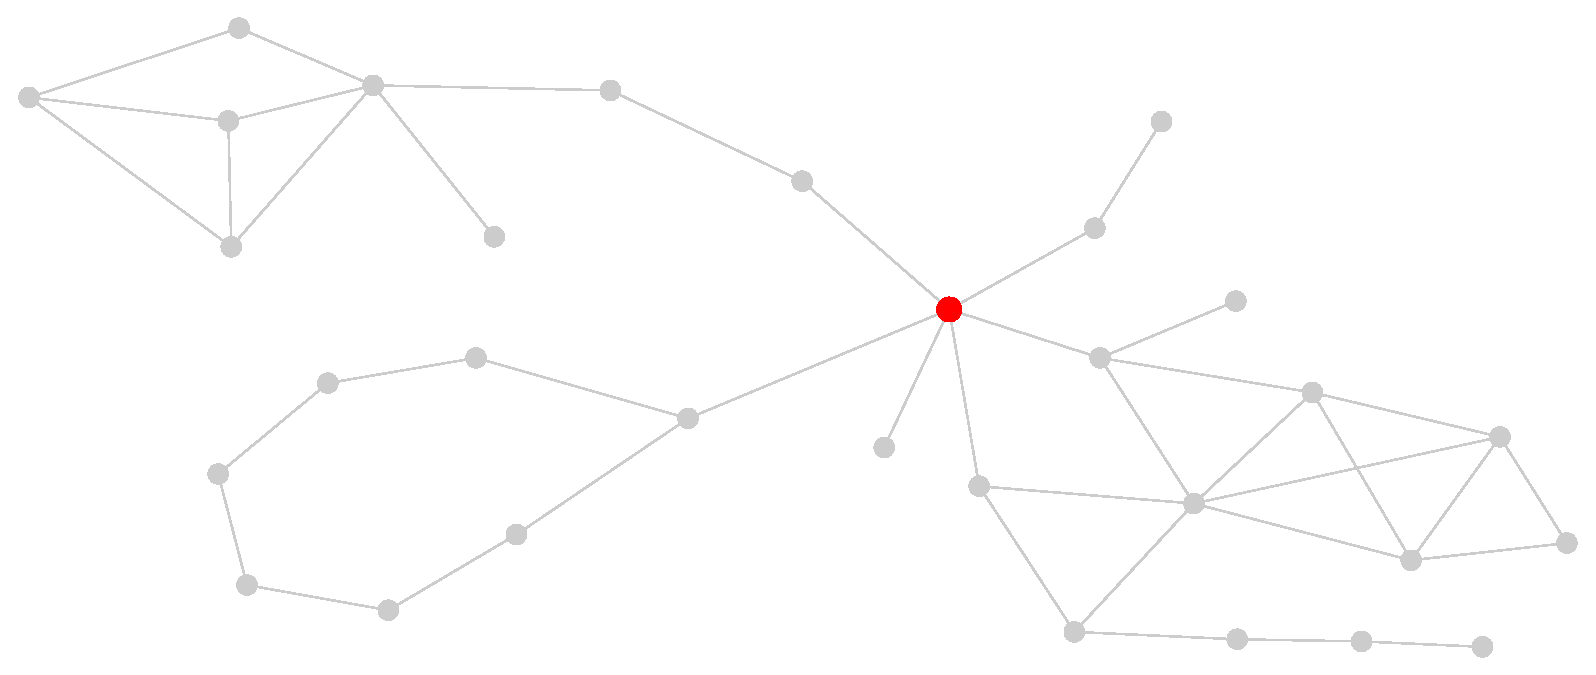
\includegraphics[width=\textwidth]{frame0}
		\caption{$k=0$}
    \label{fig:ci_diffusion_frame0}
  \end{subfigure}%
  ~
  \begin{subfigure}[b]{0.5\textwidth}
    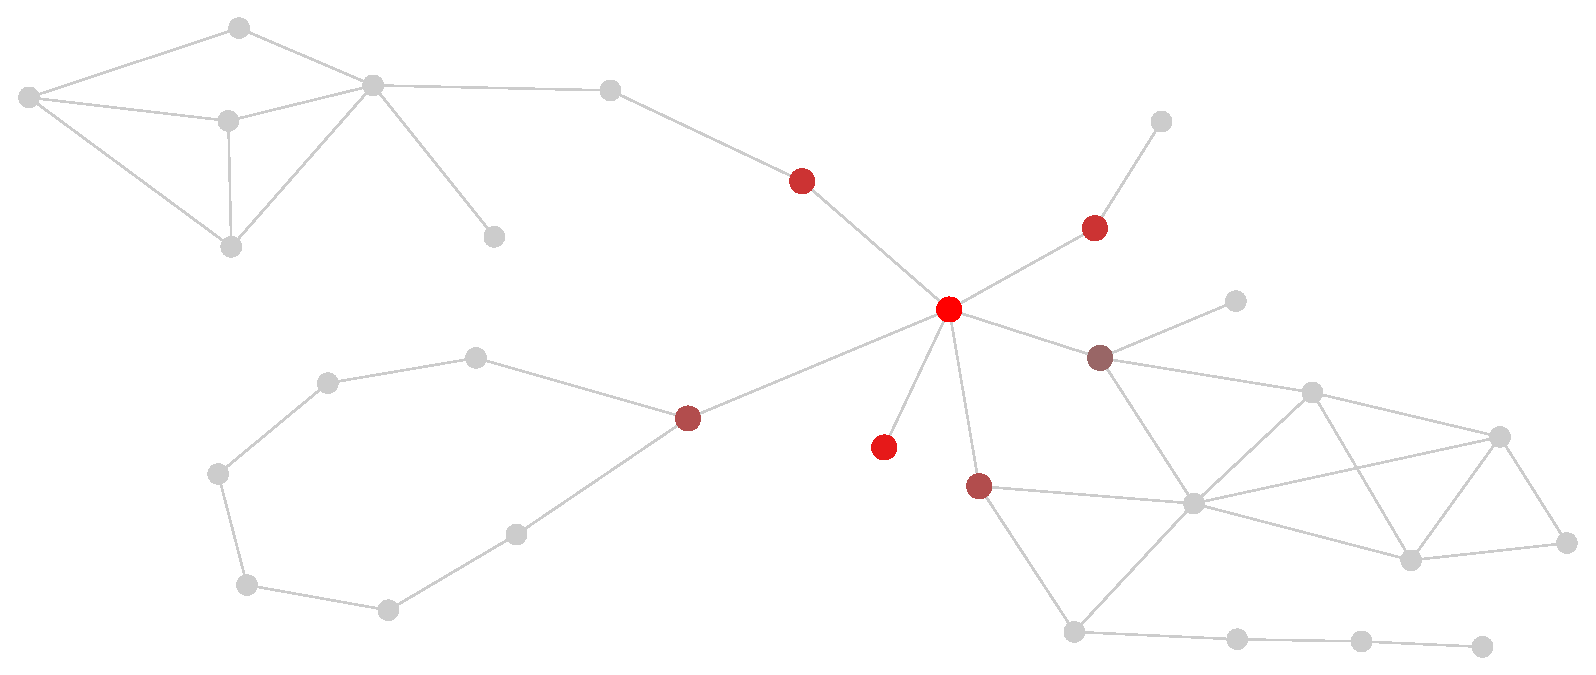
\includegraphics[width=\textwidth]{frame1}
    \caption{$k=1$}
  \end{subfigure}
  \begin{subfigure}[b]{0.5\textwidth}
    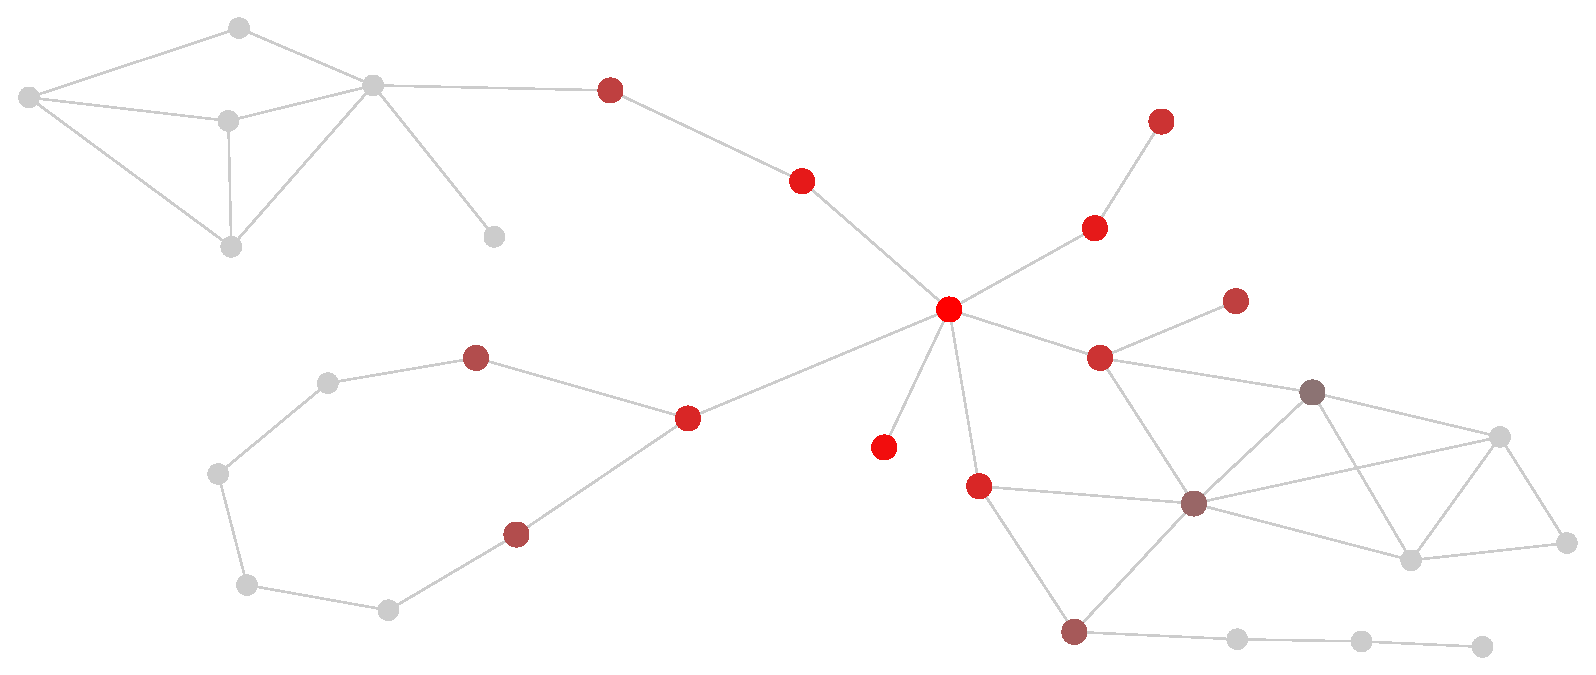
\includegraphics[width=\textwidth]{frame2}
		\caption{$k=2$}
  \end{subfigure}%
  ~
  \begin{subfigure}[b]{0.5\textwidth}
    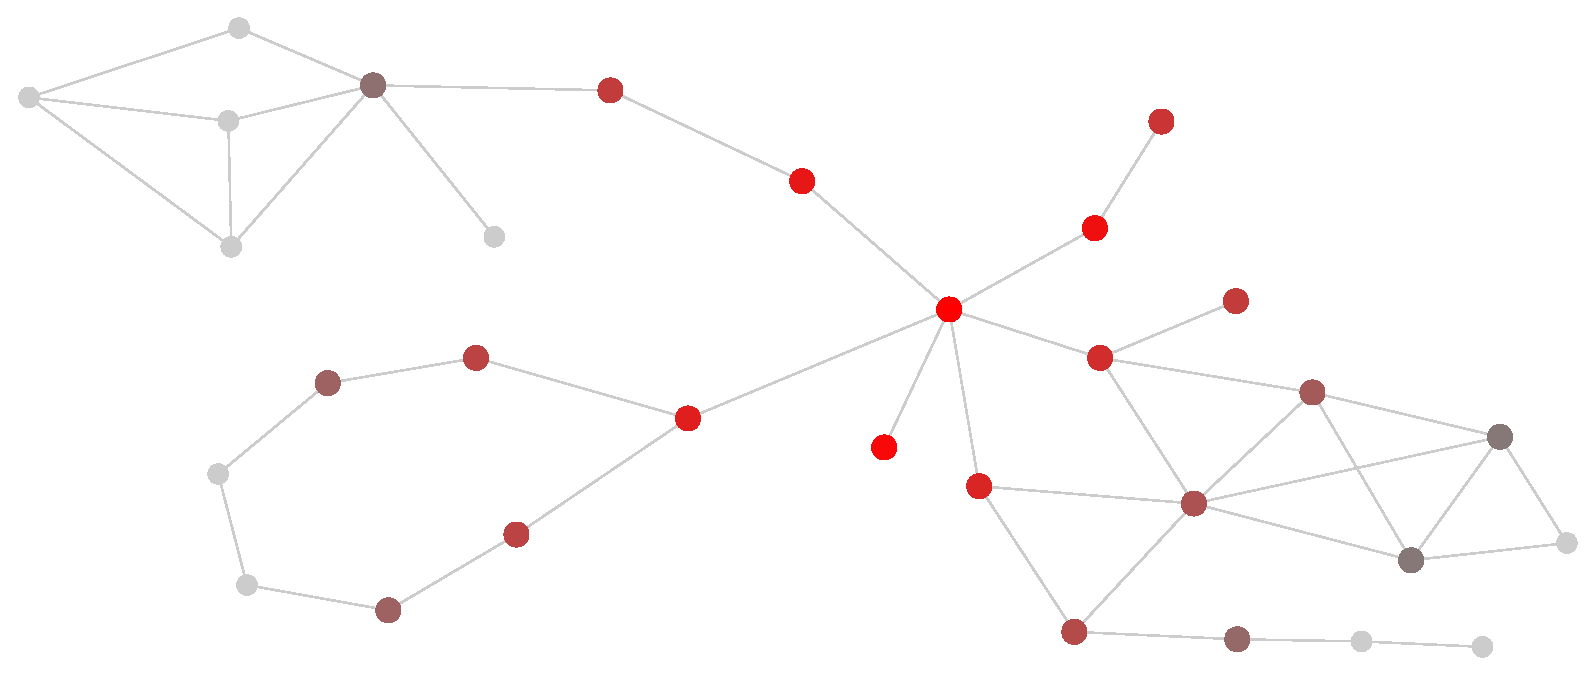
\includegraphics[width=\textwidth]{frame3}
    \caption{$k=3$}
  \end{subfigure}
  \begin{subfigure}[b]{0.5\textwidth}
    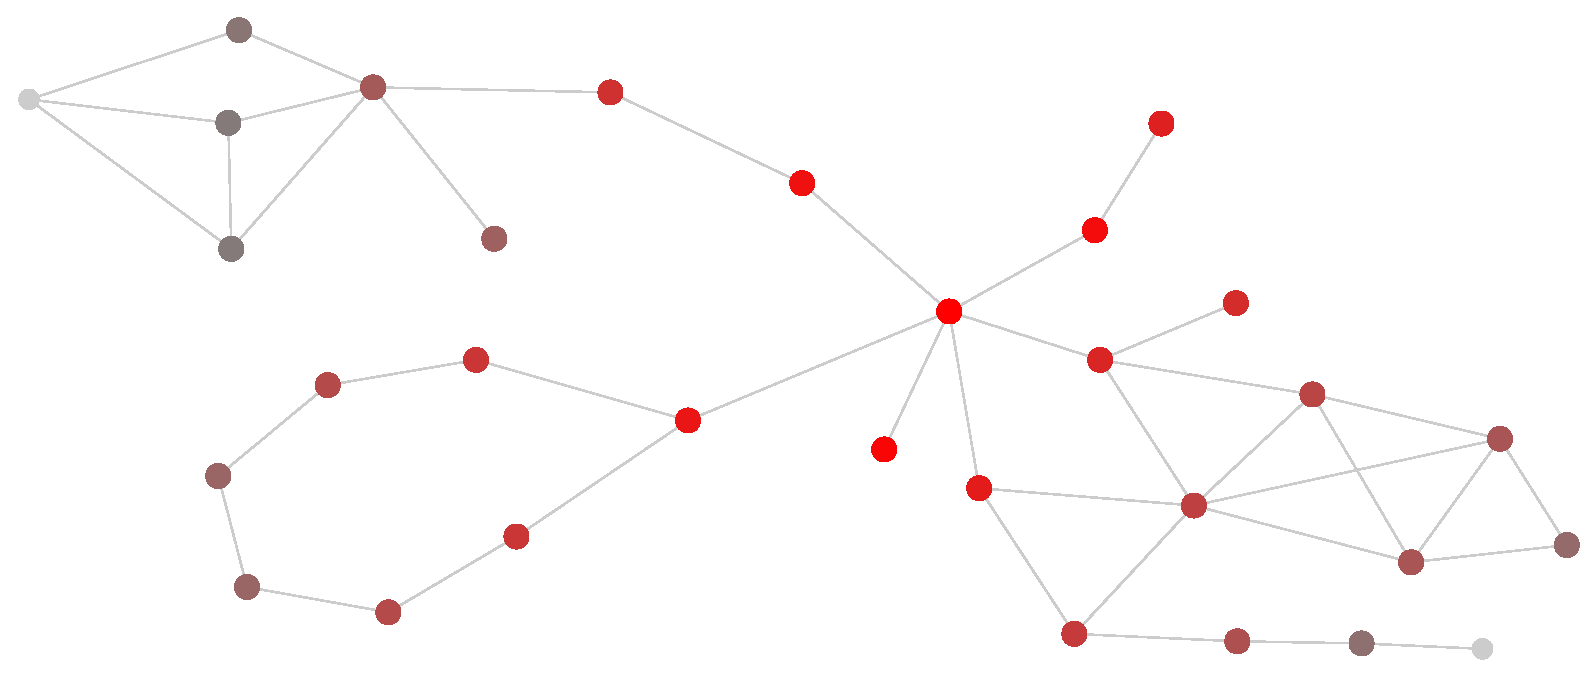
\includegraphics[width=\textwidth]{frame4}
		\caption{$k=4$}
  \end{subfigure}%
  ~
  \begin{subfigure}[b]{0.5\textwidth}
    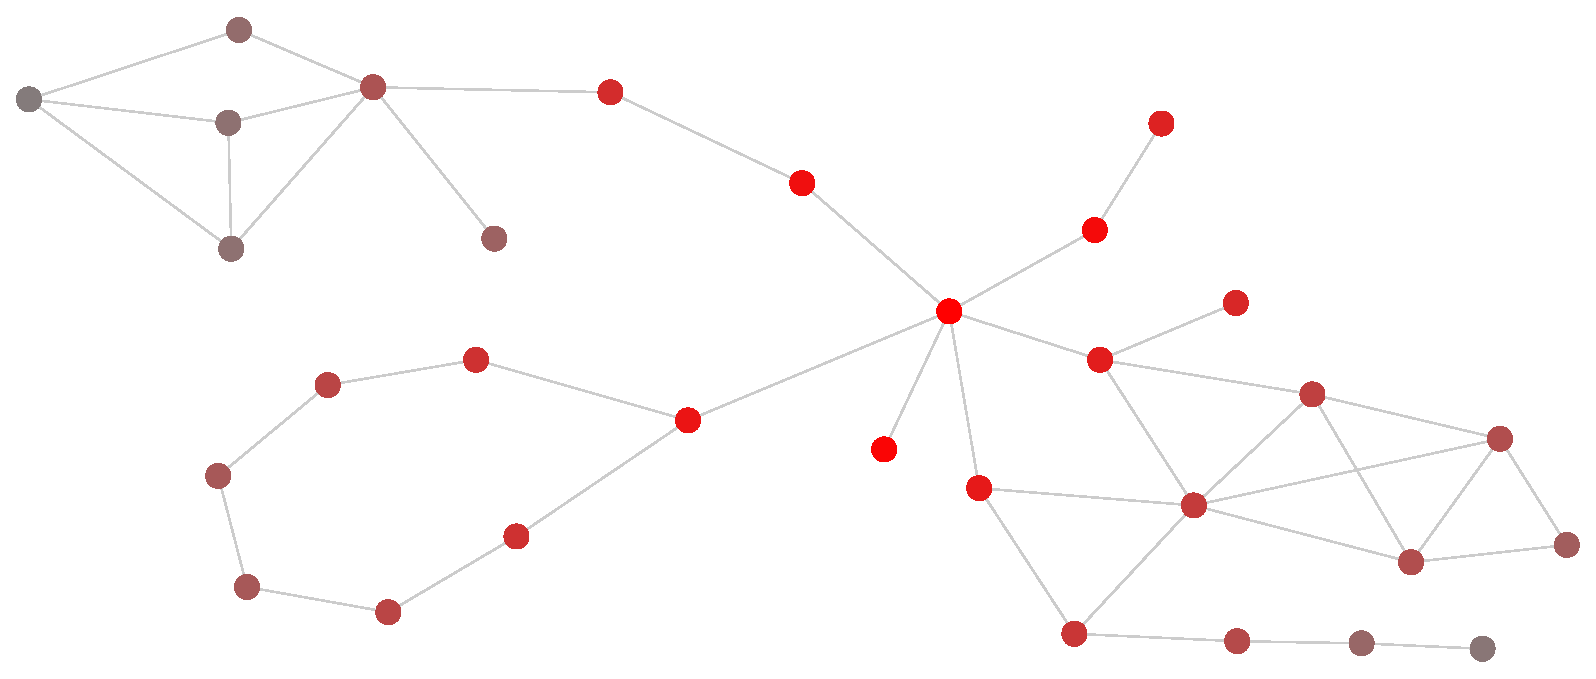
\includegraphics[width=\textwidth]{frame5}
    \caption{$k=5$}
  \end{subfigure}


  \caption{Computation of $\bm{c}_i = \sum_{t=0}^k 0.5^t \mat{D}^t \bm{\delta}_i$ up
  to different $k$. Vertex $i$ is the only red vertex in \textbf{(a)}. The
  saturation of the colour of a vertex, $j$, represents the connection strength
  between vertices $i$ and $j$ (red means strong connection and light grey no
  connection).}
  \label{fig:ci_diffusion}
\end{figure}

\subsection{Similarity between two vertices}

Two vertices of a graph are similar if they are in a similar neighbourhood. The
cloud vector of a vertex represents the neighbourhood of that vertex, therefore
the similarity between two vertices can be obtained by comparing their cloud
vectors.

One similarity measure is the Euclidean distance between cloud vectors. For
vertices $i$ and $j$ it is $\|\bm{c}_i - \bm{c}_j\|$. The smaller the distance
is, the more similar the vertices are. The minimum distance is $0$ and it is the
similarity between a vertex and itself.

Another similarity measure is the cosine similarity, which is the cosine of the
angle between the two vectors. It has values in the interval $[-1,1]$, with the
property that $\cos(0) = 1$ and $\cos(a) < \cos(b) \leq 1$, where $\pi \geq a > b
\geq 0$. A higher value means higher similarity, with $1$ being the maximum. The
cosine similarity ignores the magnitudes of the cloud vectors and only considers
the angle between them, therefore two cloud vectors that are not identical but
have the same direction (angle between them $0$) have the cosine similarity $1$.

%
%-------------------------------------------------------------------------------
% Naive implementation
%-------------------------------------------------------------------------------
%
\section{Naive approach}
%\addcontentsline{toc}{chapter}{Brute-force approach}
%
A naive implementation that does not scale to large graphs is to compute and
store all could vectors $\bm{c}_i, \forall i \in \mathcal{V}$. Observe that
\emph{Equation~\ref{eq:brute-ci}} is a geometric series and can be computed as
\begin{align}
  \label{eq:ci_inverse}
  \bm{c}_i = (\mat{I} - \mu \mat{D})^{-1} \bm{\delta}_i,
\end{align}
so every $\bm{c}_i$ vector is the $i^{th}$ column in the matrix $(\mat{I} -
\mu \mat{D})^{-1}$.

The naive approach was implemented and run on a small graph designed by hand and it gave
meaningful results (vertices connected to the graph in a similar way have a small
$\|\bm{c}_i - \bm{c}_j\|^2$) but it does not scale for large datasets.

Large graphs are expected to have sparse adjacency matrices, where the
number of edges is significantly lower then the number of vertices squared (
$|\mathcal{E}| \ll N^2$). The inverse $(\mat{I} - \mu \mat{D})^{-1}$ is
not sparse and it takes significantly more memory than the adjacency matrix. If
the graph is large enough, it can easily take more memory than the available RAM
on an average computer. Another problem is that computing the matrix inverse is
a computationally costly operation of complexity $O(N^3)$.

%
%-------------------------------------------------------------------------------
% Approximative approach
%-------------------------------------------------------------------------------
%
\section{Approximative approach}
%\addcontentsline{toc}{section}{Approximative approach}

%
%% Motivation for dot products only.
%

There are two similarity measures that should be computed, namely the Euclidean
distance between two cloud vectors and the cosine of the angle between them.

Geometrically, if vectors $\bm{c}_i$ and $\bm{c}_j$ start from the origin, then
$\bm{c}_i$, $\bm{c}_j$ and $\bm{c}_i-\bm{c}_j$ describe a triangle. Let $\theta$
be the angle between $\bm{c}_i$ and $\bm{c}_j$. From the Law of Cosines
%
\begin{equation}
  \label{eq:cosinelaw}
  \|\bm{c}_i-\bm{c}_j\|^2 = \|\bm{c}_i\|^2 + \|\bm{c}_j\|^2 - 2 \|\bm{c}_i\|
  \|\bm{c}_j\| \cos \ \theta.
\end{equation}
%
Take the dot product $\bm{c}^T_i\bm{c}_j = \| \bm{c}_i \| \| \bm{c}_j \| \cos \ \theta$.
The angle between $\bm{c}_i$ and itself is $0$ and $\cos \ 0=1$, thus
$\|\bm{c}_i\|^2 = \bm{c}^T_i\bm{c}_i$. Now \emph{Equation~\ref{eq:cosinelaw}} becomes
%
\begin{equation}
  \label{eq:norm-equation}
  \|\bm{c}_i-\bm{c}_j\|^2 = \bm{c}^T_i\bm{c}_i + \bm{c}^T_j\bm{c}_j - 2 \bm{c}^T_i\bm{c}_j,
\end{equation}
%
from which the Euclidean distance can be computed by taking the square root of the
result.

The cosine similarity can be computed using the same dot products
\begin{align}
  \cos \ \theta = \frac{\bm{c}^T_i\bm{c}_j}{\|\bm{c}_i\|\|\bm{c}_j\|} =
  \frac{\bm{c}^T_i\bm{c}_j}{\sqrt{\bm{c}^T_i\bm{c}_i} \ \sqrt{\bm{c}^T_j\bm{c}_j}}.
\end{align}

Therefore, it is sufficient to be able to compute all dot products $\bm{c}^T_i\bm{c}_j$
(for all $i, j \in v$) to compute the similarities between all vertices of the
graph. Computing and storing all $\bm{c}^T_i\bm{c}_j; i,j \in v$ takes too much
time and memory for a very large dataset, so we will make a trade-off between the
accuracy of the result and the computational complexity.


%
%% Approximative algorithm intro
%


An approximative algorithm to efficiently compute the dot products $\bm{c}^T_i\bm{c}_j$
will be described.

The algorithm is slightly different for directed and undirected graphs, because
undirected graphs have symmetric adjacency matrices. Symmetric matrices have the
advantage of having real eigenvalues and orthogonal eigenvectors, whereas
non-symmetric matrices can have both real and complex eigenvalues and the
eigenvectors need not be orthogonal.

Both versions of the algorithm use the normalised adjacency matrix (from
\emph{Equation~\ref{eq:initial-d}}), which can be vectorised as
\begin{equation}
  \label{eq:d-vectorised}
  \mat{D} = \mat{W}\mat{M},
\end{equation}
where $\mat{W}$ is the diagonal matrix
\begin{equation}
  \label{eq:W}
  \mat{W}_{ii} = \frac{1}{\sum_{j=1}^N \mat{M}_{ij}}.
\end{equation}

%
%% Undirected graphs
%

\subsection{Undirected graphs}

In this subsection, assume that the graph $\mathcal{G}$ is undirected and, as a
consequence, the adjacency matrix $\mat{M}$ is a real symmetric matrix.

The normalised adjacency matrix $\mat{D}$ is not symmetric as it is the product
of a diagonal matrix ($\mat{W}$) and a symmetric matrix ($\mat{M}$). Knowing we
are interested in $\mat{D}^t$, define a new symmetric matrix
\begin{equation}
  \label{eq:a}
  \mat{A} = \mat{W}^{\sfrac{1}{2}}\mat{M}\mat{W}^{\sfrac{1}{2}}
\end{equation}
that can be used in
\begin{align}
  \label{eq:undirected-dt-waw}
  \mat{D}^t = (\mat{W}\mat{M})^t
      = \mat{W}^{\sfrac{1}{2}} \mat{A}^t \mat{W}^{\sfrac{-1}{2}}.
\end{align}

The matrices $\mat{W}^{\sfrac{1}{2}}$ and $\mat{W}^{\sfrac{-1}{2}}$ are easy to
compute because $\mat{W}$ is a diagonal matrix. Apply the operation only on the
diagonal elements and obtain $(\mat{W}^{\sfrac{1}{2}})_{ii} = (\mat{W}_{ii})^
{\sfrac{1}{2}}$ and $(\mat{W}^{\sfrac{-1}{2}})_{ii} = (\mat{W}_{ii})^
{\sfrac{-1}{2}}$.


%
%% Defining eigen*matrices.
%


Let $\lambda_i$ be the $i^{th}$ eigenvalue of $\mat{A}$ and $\bm{\vee}^{(i)}$
its corresponding eigenvector ($\forall i \in \{ 1, 2, ..., N \}$).
$\mat{V}$ is a matrix of all $N$ eigenvectors (such that $\bm{\vee}^{(i)}$ is
the $i^{th}$ column of $\bm{\vee}$), and $\bm{\Lambda}$ is a diagonal matrix
of all $N$ eigenvalues
%
\begin{align}
  \bm{\vee} &= \begin{bmatrix}
    \vert           & \vert           &       & \vert \\
    \bm{\vee}^{(1)} & \bm{\vee}^{(2)} & \dots & \bm{\vee}^{(N)} \\
    \vert           & \vert           &       & \vert \end{bmatrix}, &&
  \bm{\Lambda} = \begin{bmatrix}
    \lambda_1 & 0 		      & \dots  & 0 \\
    0 	 	    & \lambda_2   & \dots  & 0 \\
    \vdots 	  & \vdots	    & \ddots &   \\
    0	        & 0           &        & \lambda_N
  \end{bmatrix}.
\end{align}


%
%% Eigenvalue decomposition
%


The diagonalisation of the matrix $\mat{A}$ is $\mat{A} = \bm{\vee} \bm{\Lambda}
\bm{\vee}^{-1}$.
$\mat{A}$ is a real symmetric matrix thus its eigenvectors are orthogonal, which
makes $\bm{\vee}$ an orthogonal matrix, therefore $\bm{\vee}^{-1} = \bm{\vee}^{T}$
\cite{eigval_and_eigvec}. The diagonalisation of $\mat{A}$ is then
%
\begin{align}
  \mat{A} &= \bm{\vee} \bm{\Lambda} \bm{\vee}^{T} \\
  \Rightarrow \mat{A}^t &= \big(\bm{\vee} \bm{\Lambda} \bm{\vee}^{T}\big)^t
                  = \bm{\vee} \bm{\Lambda}^t \bm{\vee}^{T} \\
  \label{eq:a-at-t-sum}
                  &= \sum_{a=1}^{N} \lambda_a^t \bm{\vee}^{(a)} \bm{\vee}^{(a)T}.
\end{align}


From \emph{Equation~\ref{eq:undirected-dt-waw}} and \emph{Equation~\ref{eq:a-at-t-sum}}
\begin{equation}
  \label{eq:d-at-t-with-a}
  \mat{D}^t = \mat{W}^{\sfrac{1}{2}} \sum_{a=1}^{N} \lambda_a^t \bm{\vee}^{(a)}
    \bm{\vee}^{(a)T} \mat{W}^{\sfrac{-1}{2}}.
\end{equation}


%
%% Plugging into the Ci
%


Plug $\mat{D}^t$ from \emph{Equation~\ref{eq:d-at-t-with-a}} into
\emph{Equation~\ref{eq:brute-ci}}
\begin{equation}
  \bm{c}_i = \sum_{t=0}^\infty \mu^t \mat{W}^{\sfrac{1}{2}} \sum_{a=1}^{N}
    \lambda_a^t \bm{\vee}^{(a)} \bm{\vee}^{(a)T} \mat{W}^{\sfrac{-1}{2}}
    \bm{\delta}_i,
\end{equation}
rearrange the equation and obtain
\begin{equation}
  \label{eq:ci-rearranged}
  \bm{c}_i = \mat{W}^{\sfrac{1}{2}} \sum_{a=1}^{N} \sum_{t=0}^\infty \mu^t
    \lambda_a^t \bm{\vee}^{(a)} \bm{\vee}^{(a)T} \mat{W}^{\sfrac{-1}{2}}
    \bm{\delta}_i.
\end{equation}


%
%% Geometric series - to look into lambda mu < 1.
%


Note that $\sum_{t=0}^\infty \mu^t\lambda_a^t$ is a sum of a geometric series
with the first term $1$ and ratio $\mu \lambda_a$, therefore
\begin{equation}
  \label{eq:geometric-series}
  \sum_{t=0}^\infty \mu^t\lambda_a^t = \frac{1}{1 - \mu \lambda_a}.
\end{equation}


Observe $\bm{\vee}^{(a)T} \mat{W}^{\sfrac{-1}{2}} \bm{\delta}_i$ is a scalar
\begin{equation}
  \label{eq:observe-scalar}
  \bm{\vee}^{(a)T} \mat{W}^{\sfrac{-1}{2}} \bm{\delta}_i =
    \bm{\vee}^{(a)}_i \mat{W}^{\sfrac{-1}{2}}_{ii}.
\end{equation}


Substitute \emph{Equation~\ref{eq:observe-scalar}} and \emph{Equation~\ref{eq:geometric-series}}
back into \emph{Equation~\ref{eq:ci-rearranged}} and obtain
\begin{equation}
  \label{eq:ci-rearranged-geometric}
  \bm{c}_i = \mat{W}^{\sfrac{1}{2}} \sum_{a=1}^{N} \frac{1}{1 - \mu \lambda_a}
    \bm{\vee}^{(a)} \bm{\vee}^{(a)}_i \mat{W}^{\sfrac{-1}{2}}_{ii}.
\end{equation}


%
%% Approximation explained.
%


An approximation of the vectors $\bm{c}_i \ (\forall i \in \mathcal{V})$ can be
obtained by only using the $k$ leading eigenvectors and eigenvalues of $\mat{A}$
instead of all of them. It is expected that the $\mat{A}$ is large and sparse,
because in a typical dataset the number of relationships is significantly
smaller than the number of data points squared. In terms of the undirected graph
$\mathcal{G}(\mathcal{V}, \mathcal{E})$, it is expected that $\|\mathcal{E}\|
\ll \|\mathcal{V}\|^2$. The Lanczos Method is an efficient iterative algorithm
to compute the leading eigenvalues of large sparse real symmetric matrices
\cite{calvetti1994implicitly} and it is implemented in both Matlab\cite{matlab:eigs} and Python
(SciPy).

Compute the largest $k$ eigenvalues and eigenvectors using the Lanczos Method
and define $\bm{\hat{\vee}}$ to be the matrix of the $k$ leading eigenvectors
and $\bm{\hat{\Lambda}}$ to be the diagonal matrix of the leading $k$
eigenvalues
\begin{align}
  \bm{\hat{\vee}} &= \begin{bmatrix}
    \vert           & \vert           &       & \vert \\
    \bm{\vee}^{(1)} & \bm{\vee}^{(2)} & \dots & \bm{\vee}^{(k)} \\
    \vert           & \vert           &       & \vert \end{bmatrix}, &&
  \bm{\hat{\Lambda}} = \begin{bmatrix}
    \lambda_1 & 0 		      & \dots  & 0 \\
    0 	 	    & \lambda_2   & \dots  & 0 \\
    \vdots 	  & \vdots	    & \ddots &   \\
    0	        & 0           &        & \lambda_k
  \end{bmatrix}.
\end{align}


Let $\bm{\hat{c}}_i$ be an approximation of $\bm{c}_i$
\begin{equation}
  \label{eq:c-hat}
  \bm{\hat{c}}_i = \mat{W}^{\sfrac{1}{2}} \sum_{a=1}^{k} \frac{1}{1 - \mu
    \lambda_a} \bm{\vee}^{(a)} \bm{\vee}^{(a)}_i \mat{W}^{\sfrac{-1}{2}}_{ii}.
\end{equation}


%
%% Define Z
%


To simplify the equation, let $\mat{Z}$ be a $N \times k$ matrix such that
\begin{align}
  \label{eq:z-ij}
  \mat{Z}_{ij} &= \frac{\bm{\vee}^{(j)}_i \mat{W}^{\sfrac{-1}{2}}_{ii}}
    {1-\mu \lambda_j},
\end{align}
or vectorised using a new $k \times k$ diagonal matrix $\mat{R}$,
\begin{align}
  \label{eq:z-vectorised}
  \mat{Z} = \mat{W}^{\sfrac{-1}{2}} \bm{\hat{\vee}} \mat{R}, &&
  \mat{R}_{ii} = \frac{1}{1 - \mu \lambda_i}.
\end{align}

Substitute $\mat{Z}$ in \emph{Equation~\ref{eq:c-hat}} to get
\begin{equation}
  \label{eq:ci-rearranged-z}
  \bm{\hat{c}}_i = \mat{W}^{\sfrac{1}{2}} \sum_{a=1}^{k} \mat{Z}_{ia}
    \bm{\vee}^{(a)}.
\end{equation}


%
%% Dot product undirected
%


The dot product between $\bm{\hat{c}}_i$ and $\bm{\hat{c}}_j$ becomes
\begin{align}
  \bm{\hat{c}}^T_i \bm{\hat{c}}_j &=
    \Big(\mat{W}^{\sfrac{1}{2}} \sum_{a=1}^{k} \mat{Z}_{ia} \bm{\vee}^{(a)} \Big)^T
    \Big(\mat{W}^{\sfrac{1}{2}} \sum_{a'=1}^{k} \mat{Z}_{ia'} \bm{\vee}^{(a')} \Big)
  \\
  &= \sum_{a=1}^{k} \mat{Z}_{ia} \bm{\vee}^{(a)T} \mat{W}
    \sum_{a'=1}^{k} \mat{Z}_{ia'} \bm{\vee}^{(a')}
  \\
  &= \sum_{a=1}^k \sum_{a'=1}^k \mat{Z}_{ia} \mat{Z}_{ja'}
    \bm{\vee}^{(a)T} \mat{W} \bm{\vee}^{(a')} \label{eq:dot-zvw}
\end{align}


%
%% Define Q
%


Define a new $k \times k$ matrix $\mat{Q}$ such that
\begin{equation}
  \label{eq:q-ij}
  \mat{Q}_{ij} = \bm{\vee}^{(i)T} \mat{W} \bm{\vee}^{(j)},
\end{equation}
or vectorised
\begin{equation}
  \label{eq:q-vectorised}
  \mat{Q} = \bm{\hat{\vee}}^T \mat{W} \bm{\hat{\vee}}.
\end{equation}

$\mat{Z}_i$ is the $i^{th}$ row of the matrix $\mat{Z}$, as a column vector.
Substitute $\mat{Q}$ into \emph{Equation~\ref{eq:dot-zvw}} and obtain
\begin{align}
  \bm{\hat{c}}_i^T \bm{\hat{c}}_j &= \sum_{a=1}^k \sum_{a'=1}^k
    \mat{Z}_{ia} \mat{Z}_{ja'} \mat{Q}_{aa'} \label{eq:dot-zq-sum} \\
  &= \mat{Z}_i^T \mat{Q} \mat{Z}_j \label{eq:dot-zq-vectorised}
\end{align}

%
%% Cholesky and positive definite Q
%

A Hermitian, positive-definite matrix can be factorised into a lower (or upper)
triangular matrix and its transpose. The process is called Cholesky decomposition.
The matrix $\mat{Q}$ only has real elements, and
\begin{align}
  \mat{Q}^T = (\bm{\hat{\vee}}^T \mat{W} \bm{\hat{\vee}})^T
    = \bm{\hat{\vee}}^T (\bm{\hat{\vee}}^T \mat{W})^T
    = \bm{\hat{\vee}}^T \mat{W} \bm{\hat{\vee}} = \mat{Q},
\end{align}
thus $\mat{Q}$ is a real symmetric matrix, so Hermitian. We expect all the
weights in the graph to be positive, so all the diagonal elements in $\mat{W}$
are positive, therefore we can say that
\begin{align}
  \forall \bm{x} \neq \bm{0},\  \bm{x}^T \mat{Q} \bm{x} &=
     (\bm{\hat{\vee}}\bm{x})^T \mat{W} (\bm{\hat{\vee}}\bm{x}) \\
     &= \sum_i \mat{W}_{ii} (\bm{\hat{\vee}}\bm{x})_i^2 > 0,
\end{align}
because $(\bm{\hat{\vee}}\bm{x}) = \bm{0}$ if and only if $\bm{x} = \bm{0}$
since $\bm{\hat{\vee}}$ is orthogonal. Therefore, by definition, $\mat{Q}$ is
positive definite.

Using Cholesky decomposition, $\mat{Q}$ can be written as $\mat{Q} = \mat{L}
\mat{L}^T$, which can be used to simplify the dot product even further as
follows
\begin{align}
  \bm{\hat{c}}_i^T \bm{\hat{c}}_j &= \mat{Z}_i^T \mat{L} \mat{L}^T \mat{Z}_j \\
   &= (\mat{L}^T \mat{Z}_i)^T (\mat{L}^T \mat{Z}_j).
\end{align}

Define a new $k \times N$ matrix $\bm{\omega}$ with columns
$\bm{\omega}_i = \mat{L}^T \mat{Z}_i$, which can be vectorised as
\begin{equation}
  \bm{\omega} = \mat{L}^T \mat{Z}^T.
\end{equation}

The final form of the approximative dot product between cloud vectors is
\begin{equation}
  \bm{\hat{c}}_i^T \bm{\hat{c}}_j = \bm{\omega}_i^T \bm{\omega}_j,
\end{equation}
therefore the only matrix that needs to be computed and stored is $\bm{\omega}$,
which takes $O(kN)$ space. Computing an approximative dot product has the time
complexity $O(k)$, because the only operation is a dot product of two vectors of
size $k$.

In the rest of this report, we will refer to a computed $\mat{\omega}$ as an
\emph{undirected index}, because it is the only matrix required to compute all
the relevant similarity measures for an undirected graph.

%% TODO: time complexity analysis of training: lanczos method and cholesky


%
%% Directed graphs
%

\subsection{Directed graphs}

In this subsection, assume that the graph $\mathcal{G}$ is directed and, as a
consequence, the adjacency matrix $\mat{M}$ is a general real matrix. As
$\mat{M}$ is not symmetric, there is no property to take advantage of, thus
the normalised adjacency $\mat{D}$ will be used directly.

Let $\bm{\Lambda}$ be a diagonal matrix with the eigenvalues of $\mat{D}$, where
$\lambda_i$ is the $i^{th}$ eigenvalue. $\bm{\vee_R}^{(i)}$ is the $i^{th}$
right eigenvector and $\bm{\vee_R}$ is a matrix of the right
eigenvectors. $\bm{\vee_L}^{(i)}$ is the $i^{th}$ left eigenvector and
$\bm{\vee_L}$ is a matrix of the left eigenvectors.
\begin{align}
  \bm{\vee_R} &= \begin{bmatrix}
    \vert           & \vert           &       & \vert \\
    \bm{\vee_R}^{(1)} & \bm{\vee_R}^{(2)} & \dots & \bm{\vee_R}^{(N)} \\
    \vert           & \vert           &       & \vert \end{bmatrix}, &&
  \bm{\vee_L} &= \begin{bmatrix}
      \horz   & \bm{\vee_L}^{(1)} & \horz \\
      \horz   & \bm{\vee_L}^{(2)} & \horz \\
              & \vdots            &       \\
      \horz   & \bm{\vee_L}^{(N)} & \horz \end{bmatrix}, &&
  \bm{\Lambda} = \begin{bmatrix}
    \lambda_1 & 0 		      & \dots  & 0 \\
    0 	 	    & \lambda_2   & \dots  & 0 \\
    \vdots 	  & \vdots	    & \ddots &   \\
    0	        & 0           &        & \lambda_N
  \end{bmatrix}.
\end{align}

Some of the eigenvalues and some elements of the eigenvectors might be complex.
However, because $\mat{D}$ is real, if an eigenvalue $\lambda_i$ is complex,
there exists an eigenvalue $\lambda_j$ that is its complex conjugate, that is
$\lambda_i = \conj{\lambda_j}$. The same applies to eigenvectors, if an
eigenvector $\bm{\vee}^{(i)}$ (left or right) has complex elements, there exists
another eigenvector $\bm{\vee}^{(j)}$ (left or right, respectively) that is its
complex conjugate, $\bm{\vee}^{(i)} = \conj{\bm{\vee}^{(j)}}$.

Knowing that $\bm{\vee_R}^{-1} = \bm{\vee_L}$, the eigendecomposition of
$\mat{D}$ is
\begin{equation}
  \mat{D} = \bm{\vee_R} \bm{\Lambda} \bm{\vee_R}^{-1}
          = \bm{\vee_R} \bm{\Lambda} \bm{\vee_L}.
\end{equation}
Also
\begin{equation}
  \mat{D}^t = \bm{\vee_R} \bm{\Lambda}^t \bm{\vee_R}^{-1}
            = \bm{\vee_R} \bm{\Lambda}^t \bm{\vee_L}.
\end{equation}

We can now write $\bm{c}_i$ as
\begin{align}
  \bm{c}_i &= \sum_{t=0}^\infty \mu^t \mat{D}^t \bm{\delta}_i \\
   &= \sum_{t=0}^\infty \mu^t \bm{\vee_R} \bm{\Lambda}^t \bm{\vee_L}
      \bm{\delta}_i \\
   &= \sum_{t=0}^\infty \mu^t \sum_{a=1}^N \lambda_a^t \bm{\vee_R}^{(a)}
      \bm{\vee_L}^{(a)} \bm{\delta}_i.
\end{align}
Note that $\bm{\vee_L}^{(a)} \bm{\delta}_i$ is the $i^{th}$ value of
$\bm{\vee_L}^{(a)}$ and obtain
\begin{equation}
  \bm{c}_i = \sum_{t=0}^\infty \mu^t \sum_{a=1}^N \lambda_a^t \bm{\vee_R}^{(a)}
     \bm{\vee}_{\bm{L}i}^{(a)}.
\end{equation}
Observe that $\sum_{t=0}^\infty \mu^t \lambda_a^t$ is a sum of a geometric
series, rearrange and obtain
\begin{equation}
  \bm{c}_i = \sum_{a=1}^N \frac{\bm{\vee}_{\bm{L}i}^{(a)}}
             {1 - \mu \lambda_a} \bm{\vee_R}^{(a)}.
\end{equation}

Same as for undirected graphs, an approximation of the cloud vectors can be made
using only a small number of the largest eigenvalues and eigenvectors. Because
$\mat{D}$ is not symmetric, it might have complex eigenvalues, and in order to
have real approximations of the cloud vectors, it is necessary to check that for
every complex eigenvalue used its complex conjugate is also used.


Let $\bm{\hat{\Lambda}}$ be a diagonal matrix containing the leading $k$
eigenvalues, $\bm{\hat{\vee}_R}$ be a matrix that contains the leading $k$ right
eigenvectors, and $\bm{\hat{\vee}_L}$ a matrix of the leading $k$ left
eigenvectors. Arnoldi Iteration is an efficient iterative algorithm to compute
the leading eigenvalues and eigenvectors of large sparse matrices
\cite{lehoucq1996deflation}. Assume that in the $k$ eigenpairs computed, if
there is a complex eigenvalue $\lambda_i$, there also is its complex conjugate,
$\lambda_j = \conj{\lambda_i}$.


Let $\bm{\hat{c}}_i$ be the approximation of the cloud vector $\bm{c}_i$,
\begin{equation}
  \label{eq:directed-hat-ci}
  \bm{\hat{c}}_i = \sum_{a=1}^k \frac{\bm{\vee}_{\bm{L}i}^{(a)}}
             {1 - \mu \lambda_a} \bm{\vee_R}^{(a)}.
\end{equation}

For any complex number $x = a+bi$, the sum $x + \conj{x} = a + bi + a - bi =
2a$ is real. The approximative cloud vectors $\bm{\hat{c}}_i$ are real vectors
because they are sums of real numbers and pairs of complex and complex
conjugates, as
\begin{align}
  \label{eq:directed-ci-real}
  \text{for all } \lambda_a \in \mathbb{C}-\mathbb{R} \
    &\text{there exists } \lambda_b = \conj{\lambda_a}
    \text{ such that} \ b \leq k, \\
  \text{for all } \bm{\vee}_{\bm{L}i}^{(a)} \in \mathbb{C}-\mathbb{R} \
    &\text{there exists } \bm{\vee}_{\bm{L}i}^{(b)} = \conj{\bm{\vee}_{\bm{L}i}^{(a)}}
    \text{ such that} \ b \leq k, \\
  \text{for all } \bm{\vee_R}^{(a)} \in \mathbb{C}-\mathbb{R} \
    &\text{there exists } \bm{\vee_R}^{(b)} = \conj{\bm{\vee_R}^{(a)}}
    \text{ such that} \ b \leq k.
\end{align}
The assumption about $k$ only covers the first rule
(\emph{Equation~\ref{eq:directed-ci-real}}) but it is sufficient because an
eigenvector is complex only if its corresponding eigenvalue is complex and
if two eigenvalues are conjugates $\lambda_a = \conj{\lambda_b}$ then their
corresponding eigenvectors are also conjugates $\bm{\vee}^{(a)} =
\conj{\bm{\vee}^{(b)}}$.

%
%% (Directed) Define Z
%

\emph{Equation~\ref{eq:directed-hat-ci}} can be rewritten as
\begin{equation}
  \bm{\hat{c}}_i = \sum_{a=1}^k \mat{Z}_{ia} \bm{\vee_R}^{(a)},
\end{equation}
where $\mat{Z}$ is a $N \times k$ matrix such that
\begin{equation}
  \mat{Z}_{ij} = \frac{\bm{\vee}_{\bm{L}i}^{(j)}}{1 - \mu \lambda_j},
\end{equation}
or vectorised using a new $k \times k$ diagonal matrix $\mat{R}$,
\begin{align}
  \label{eq:directed-z-vectorised}
  \mat{Z} = \bm{\hat{\vee}_L}^T \mat{R}, &&
  \mat{R}_{ii} = \frac{1}{1 - \mu \lambda_i}.
\end{align}

The dot product between $\bm{\hat{c}}_i$ and $\bm{\hat{c}}_j$ becomes
\begin{align}
  \bm{\hat{c}}_i^T \bm{\hat{c}}_j &=
        \Big( \sum_{a=1}^k \mat{Z}_{ia} \bm{\vee_R}^{(a)} \Big)^T
        \Big( \sum_{a'=1}^k \mat{Z}_{ja'} \bm{\vee_R}^{(a')} \Big) \\
  \label{eq:directed-ci-z}
  &= \sum_{a=1}^k \sum_{a'=1}^k \mat{Z}_{ia} \mat{Z}_{ja'}
        \bm{\vee_R}^{(a)T} \bm{\vee_R}^{(a')}
\end{align}

%
%% (Directed) Define Q
%

Define a $k \times k$ matrix $\mat{Q}$ such that
\begin{equation}
  \mat{Q}_{ij} = \bm{\vee_R}^{(i)T} \bm{\vee_R}^{(j)},
\end{equation}
or vectorised
\begin{equation}
  \mat{Q} = \bm{\hat{\vee}_R}^T \bm{\hat{\vee}_R},
\end{equation}
and substitute it into the dot product (\emph{Equation~\ref{eq:directed-ci-z}})
to obtain
\begin{equation}
  \bm{\hat{c}}_i^T \bm{\hat{c}}_j = \sum_{a=1}^k \sum_{a'=1}^k
    \mat{Z}_{ia} \mat{Z}_{ja'} \mat{Q}_{aa'}.
\end{equation}

$\mat{Z}_i$ is the $i^{th}$ row of the matrix $\mat{Z}$, as a column vector.
The final approximative dot product between two cloud vectors in a directed
graph is then
\begin{equation}
  \bm{\hat{c}}_i^T \bm{\hat{c}}_j = \mat{Z}_i^T \mat{Q} \mat{Z}_j.
\end{equation}

In this case, Cholesky decomposition cannot be applied because $\bm{\hat{\vee}}$
is not orthogonal and, as a consequence, $\mat{Q}$ is not positive-definite.

It is only required to compute and store $\mat{Q}$ and $\mat{Z}$, which together
take $O(k^2+kN)$ space. The time complexity of computing the approximative dot
product between two cloud vectors is the same as multiplying two vectors of
length $k$ and a $k \times k$ matrix.

In the rest of this report, we will refer to a computed pair of matrices
$\mat{Q}$ and $\mat{Z}$ as a \emph{directed index}.

%
%% Comparison with naive
%

\subsection{Comparison with naive approach}

While the naive approach takes significantly more time and space ($O(N^3)$ space
compared to $O(k^2 + kN)$), it also represents the graph more accurately because
it uses the whole adjacency matrix and not only an approximation of it.

A simple evaluation metric of how well the approximative approach retains the
most important information from the graph is to evaluate how different are the
top similar vertices for the naive approach and the approximative approach
with different choices of $k$.


For a dataset of $N$ vertices, let $B(i,j)$ be the position of vertex $j$ in
the top similar vertices of vertex $i$ for the naive approach. Similarly, let
$T_k(i,j)$ be the position of vertex $j$ in the top similar vertices of vertex
$i$ for the approximative approach with $k$ eigenvalues. Define the difference
between two such tops to be
\begin{equation}
  d(B, T_k) = \frac{1}{N^3}
    \sum_{i=1}^N \sum_{j=1}^N \operatorname{abs}(B(i,j) - T_k(i,j)).
\end{equation}
The equation is normalised by $N^3$ because the maximum value we can get lies in
the interval $(N^2, N^3)$.
%
\begin{figure}[tpb]
        \centering
        \begin{subfigure}[b]{0.6\textwidth}
	        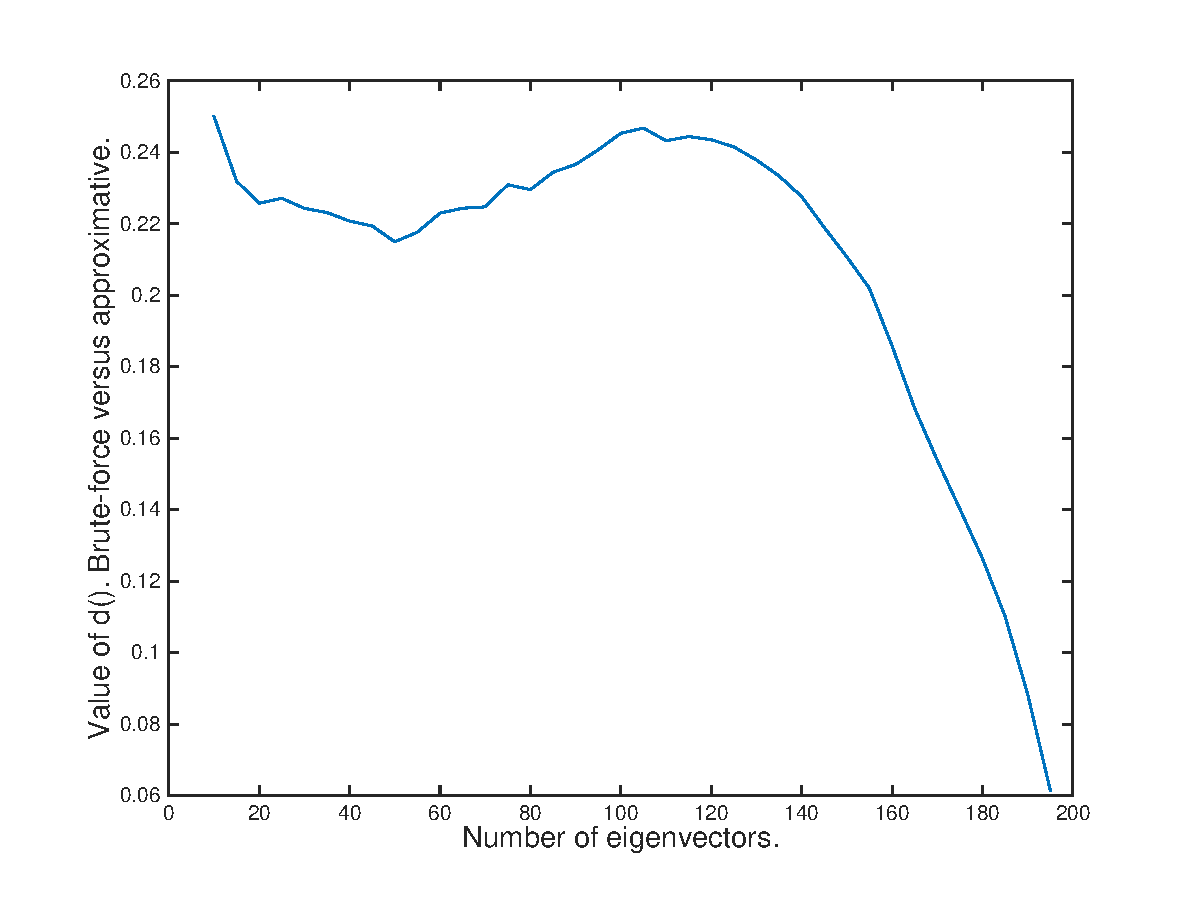
\includegraphics[width=\textwidth]{no-of-eigenvectors}
        		\caption{A plot of the differences on a range of eigenvalues.}
        \end{subfigure}%
        ~
        \begin{subfigure}[b]{0.4\textwidth}
           \centering
           \def\arraystretch{1.5}
           \begin{tabular}{|c|c|}
	   \hline
	   Parameters & Value of d() \\
	   \hline
	   $d(B, T_{10})$ & 0.2501 \\
	   \hline
	   $d(B, T_{20})$ & 0.2257   \\
	   \hline
   	   $d(B, T_{30})$ & 0.2243   \\
	   \hline
	   $d(B, T_{40})$ & 0.2208   \\
	   \hline
	   $d(B, T_{50})$ & 0.2150 \\
	   \hline
	   $d(B, T_{100})$ & 0.2453\\
	   \hline
	    $d(B$, $T_{199})$ & 0.0325 \\
	    \hline
	   \end{tabular}
	   \caption{Table of some of the values.}
	   \label{tbl:comparisons}
        \end{subfigure}%
        \caption{Difference of results between naive and approximative approaches.}
	\label{fig:no-of-eigenvectors}
\end{figure}
%


The value of $d()$ was evaluated on a randomly generated undirected graph with
$200$ vertices and $350$ edges, between the naive approach
and the approximative approach with $k = 10, 11, \dots, 199$ eigenvectors. The
choice of the penalising factor $\mu=0.5$ was used for all the runs. The results
can be observed in \emph{Figure~\ref{fig:no-of-eigenvectors}}. We can see that
if we use the majority of eigenvalues, the value of $d()$ is very small. It is
computationally infeasible to do that on a large dataset thus we will aim for a
number of eigenvectors $k$ in the range of $20$ to $40$, where the difference
seems to be at a local minimum (for this graph). The local minimum differs from
dataset to dataset depending mainly on the size of the dataset. For completeness,
the experiment was run on a randomly generated undirected graph with $500$
vertices and $700$ edges. The first local minimum of $d()$ was at around $100$
eigenvectors with a value of approx. $0.2$. At $40$ and $20$ eigenvectors, the
values of $d()$ obtained are $0.2297$ and $0.2557$, respectively.


This is just an evaluation of how well the approximation performs compared to
the naive implementation. However, on real datasets it might be the case that
ignoring some information is better than using it and the approximation approach
might perform better. For large enough datasets it is impossible to compute the
exact similarities.

%
%% Heuristics and the n^2 comparisons
%

\section{Heuristics and the $N^2$ comparisons}

After having a directed or undirected index, thus a fast way of computing the
dot products between cloud vectors and the relevant similarity measures, it is
still required to compute the similarities between all the vertices in the graph
to obtain the pairs of top similar vertices, which is a task of complexity
$O(kN^2+2N^2\log N)$ (computing all similarities and sorting). For some
applications like recommender systems, evaluating the top similarities on demand
for one vertex at a time and having a good cache will save some computing power,
however it is still a $O(kN+N\log N)$ task for every cache miss, which might be
too slow for large systems that require a constant low latency.


Assume that if two vertices are too far away from each other in the graph, they
are unlikely to be similar. The computation of similarities can then be limited
to only those pairs of vertices that are not too far away. Formally, let
$\operatorname{dist}(i,j)$ be the distance between vertices $i$ and $j$ (the
length of the shortest path). Only compute similarities for those pairs of
vertices such that $\operatorname{dist}(i, j) \leq d$ for $d$ being the maximum
distance allowed, and consider all the other pairs of vertices not similar. This
filter is implemented using a trivial breadth first search stopping at the
desired maximum depth.


We will call the filter applied on the graph to drop pairs of edges that are
unlikely to be similar a \emph{heuristic}, and the maximum distance filter
described above will be called the \emph{maximum depth heuristic}.


Using a heuristic can reduce the number of similarities computed and thus speed
up the computation while not having a big impact on the overall accuracy. As an
example, on a friends dataset of $4039$ vertices, $83,822$ edges and a diameter
of $8$ (longest shortest path), the maximum depth heuristic with depth 3 has
reduced the number of comparisons by approx. $36.3\%$, and the overall change in
accuracy is negligible. The evaluation of the algorithm on the SNAP Facebook
dataset (on a range of $k$ and $\mu$) with no heuristic takes about $37$
minutes, and with the maximum depth heuristic of depth $3$, it only takes about
$18$ minutes (approx. $2x$ speed-up).

%
%-------------------------------------------------------------------------------
% IMPLEMENTATION
%-------------------------------------------------------------------------------
%
\section{Implementation}
%\addcontentsline{toc}{section}{Implementation}
%


\newenvironment{methodListC}[2]{
  \newcommand{\mtd}[2]{\texttt{##1} & ##2 \\}
  \newcommand{\mtdfootCaption}{#2}
  \newcommand{\mtdfootLabel}{#1}
  \begin{table}[!ht]
    \centering
    \begin{tabular}{lp{10cm}}
}{
\end{tabular}
\caption{\mtdfootCaption}
\label{\mtdfootLabel}
\end{table}
}

\newenvironment{methodList}{
  \newcommand{\mtd}[2]{\texttt{##1} & ##2 \\}
  \begin{table}[!ht]
    \centering
    \begin{tabular}{lp{10cm}}
}{
\end{tabular}
\end{table}
}

\subsection{Early versions}

At the beginning of the project, a choice had to be made on what tools and
languages to use for the implementation of this algorithm. At a very early stage
the requirement was a language that provides easy interfaces to common and not
very common linear algebra functions and algorithms. Matlab was picked because
it has all the common matrix operations, good sparse matrix support and all the
eigenvalue algorithms required built-in. Matlab is also easy to prototype in.


The approximative approach for undirected graphs was implemented in Matlab as a
couple of functions. The function signatures along with descriptions are
presented in \emph{Table~\ref{tbl:matlab-interface}}. Some helper functions are
not included in the table. The (iterative) naive algorithm was implemented as a
separate set of Matlab functions with a very similar interface.

\begin{methodListC}{tbl:matlab-interface}{Matlab implementation interface.}
  \mtd{similarity(adj, mu, k)}{Computes and returns matrices $\mat{Q}$ and
    $\mat{Z}$.}
  \mtd{sim2(q, z, i, j)}{Computes the similarity between vertices i and j.}
  \mtd{simlist(q, z, i)}{Computes the similarity between vertex i and all other
    vertices.}
  \mtd{top(q, z, i)}{Uses simlist(q,z,i) and sorts the results.}
  \mtd{randomGraph(v, e, dir)}{Generates a random connected graph with v
    vertices and e edges. If dir==true, the graph is directed, otherwise it is
    undirected. }
\end{methodListC}

Matlab is, however, not very good at handling different types of files, loops,
and general data wrangling. It also cannot be easily used from the command line
or from other languages which is very useful for data processing and for
incorporating the algorithm in larger systems.

\subsection{Data processing tools}

In an ideal world, the data comes in the exact format that we want.
Unfortunately, this is never the case in the real world where data comes in all
shapes and sizes and thus there is a need for tools to process it, and reshape
it to fit into the system.


In the Matlab model, a graph file could be a CSV file where each row represents
an edge, and each vertex is an integer starting from 1 and incrementing. Nearly
no real world dataset comes in this format and in order to make the conversion
some tools must be implemented.


The tools should be quick and easy to use and simple to change and adapt if the
requirements change, thus it is best if they are small command line programs
that are good at doing one task each. A good language for writing data wrangling
tools is simple, easy to compile and run, easy to prototype in and has a good
standard library for I/O and parsing common file formats. Go was picked due to
my fluency in the language and because it fits all the requirements for writing
such tools.


A way to parse an input dataset to CSV edge lists was required. The tools are
different from dataset to dataset, and the implementations can vary from small
Go programs to bash scripts, depending on the input formats.


After the dataset is in CSV format, a tool is needed to make the vertex IDs
integers from 1 to N (the number of vertices). A command line tool called
\emph{autoincr} was implemented in Go. It takes one or more CSV edge lists and
assigns each vertex an integer ID starting from one and incrementing. It also
stores a JSON file with the mappings created so the original vertex names can be
looked up. The help message of the command line tool explains how it works in
more detail.


Given a CSV edge list file, it was necessary to be able to easily find basic
information about the graph it describes, like how many connected components it
has, whether it is directed or undirected, the number of vertices, the number of
edges. It was also required to be able to manipulate these graphs easily with
actions like forcing a directed graph to be undirected (by adding the missing
reverse edges), splitting a disconnected graph into more graphs, one for each
connected component, and removing random edges from a connected graph while
keeping it connected. The command line tool \emph{conncomp} was written in Go
for this purpose. The tool is used like this (snippet from the help message):

\begin{lstlisting}
  conncomp -action <action> [flags] <list of edge lists>

  Possible actions:

  details           Output details about the graphs.
  components        Splits the graph(s) in connected components.
  remove -n P       Removes at most P% random edges from graph(s).
  force-undirected  Force the graph(s) into undirected graph(s).
\end{lstlisting}

Unit tests were written for both \emph{conncomp} and \emph{autoincr}.

All the tools described in this section are publicly available on GitHub under
the MIT licence. The URL of the repository is
\url{https://github.com/vladvelici/graph-dataset-tools}.

\subsection{Python, SciPy and NumPy}

After starting to process a real-world dataset for the evaluation of this
algorithm, it turns out that Matlab was not the best choice for a couple of
reasons:

1. It is very hard to write command line tools and they are slow to run because
they need to open Matlab before running the scripts. This could be solved by
using Octave to run the existing Matlab codebase, but it would not solve the
other limitations.

2. The language is designed for linear algebra tasks, and it is inconvenient and
non-intuitive to implement even simple graph algorithms in it.

3. It is hard to integrate the Matlab scripts into another system (e.g. a
web service for building an interactive visualisation for the algorithm).


Other languages were investigated to port the algorithm in. The first one to
look at was Go because some tools were already written in Go. There are some
libraries for linear algebra in Go (e.g. bigo.matrix \cite{biogo} which uses
BLAS, or skelterjohn/go.matrix \cite{go.matrix} which has parallel matrix
multiplication implemented), but they are not mature enough and do not have
(or have very limited) support for sparse matrices and eigenvalue/eigenvector
computations.

Linear algebra libraries for C++ were also investigated. SLEPc \cite{slepc} is a
mature library for large sparse eigenvalue problems implemented as an extension
of PETSc \cite{petsc}. It includes implementations of the Lanczos Method and
Arnoldi Iteration, however the interfaces are very low level and prototyping
using it would be too slow.

Armadillo \cite{armadillo} is another C++ linear algebra library. It has a high
level API backed by efficient implementations of all the basic matrix operations.
It also has support for sparse matrices and computation of leading eigenvalues
and eigenvectors. The API Armadillo provides is very similar to Matlab, making
the algorithm easier to port.

The last language and set of libraries analysed is Python with NumPy and SciPy
\cite{scipy}. Python is a scripting language that is easy to read and write and
can be used interactively. SciPy is a mature scientific computing library for
Python which contains all the basic linear algebra functions, has good support
for sparse matrices and uses ARPACK (same as Matlab and Armadillo) to access
efficient implementations of the Lanczos Method and the Arnoldi Iteration. It
also has a very good and accessible documentation, a relatively large user base
and active community.

A choice had to be made on which of these tools to use. C++ with Armadillo and
Python with NumPy and SciPy were the best options in terms of linear algebra
support and ease of use. Simple code was written in C++ with Armadillo and it
turned out that routine parts of the code like parsing CSV files, dealing with
I/O and command line flags were taking too long to write. In Python these tasks
are trivial and the Python Standard Library has parsers for plenty of file
formats and command line flag parsers. The interactive shell was also very handy
to try things out before implementing them in a larger codebase.

As a result, Python with NumPy and SciPy were chosen to port the algorithm and
continue the development.

\subsection{Final implementation}

The final implementation is based on two simple concepts. A similarity index,
called a {\tt Sim} object and a provider ({\tt Provider}).

In the package {\tt sim}, the class {\tt Sim} represents a directed or undirected
index. A list of methods is in \emph{Table~\ref{tbl:sim-methods}}. Internally,
a {\tt Sim} object has either a $\bm{\omega}$ matrix or a pair of $\mat{Q}$ and
$\mat{Z}$, which it uses to compute the dot products and the similarities. The
implementation of {\tt Sim.nib(a)} is simply returning {\tt a}. This is because
the {\tt Sim} class represents an index directly trained from an adjacency
matrix but, in practice, vertices usually come with different IDs, strings or
integers that are not necessarily consecutive.

\begin{methodListC}{tbl:sim-methods}{Methods of class {\tt Sim}.}
  \mtd{\_dotprod(a, b)}{Computes the dot product between vertices {\tt a} and {\tt b}.}
  \mtd{score(a, b)    }{Computes the Euclidean distance squared.}
  \mtd{save(f)        }{Writes the index into file {\tt f}.}
  \mtd{nodelist()     }{Returns a list of all vertices.}
  \mtd{nid(a)         }{Returns the index of vertex {\tt a} in the index.}
  \mtd{\_\_len\_\_()  }{Returns the number of vertices.}
\end{methodListC}

The class {\tt Simp} extends the class {\tt Sim}. A {\tt Provider} is required
to promote an object of type {\tt Sim} to {\tt Simp}. Any object that can create
an adjacency matrix and a mapping from any (relevant) type of vertex ID to an
integer index in the adjacency matrix is a {\tt Provider}. The list of methods
an object is required to implement to be a {\tt Provider} is in
\emph{Table~\ref{tbl:provider-methods}}.

\begin{methodListC}{tbl:provider-methods}{List of methods required for an object
  to have to be a valid {\tt Provider}.}
  \mtd{\_\_getitem\_\_(a)}{Get the index of {\tt a} in the adjacency matrix.}
  \mtd{\_\_len\_\_()     }{Return the number of vertices.}
  \mtd{adj()         }{Get the adjacency matrix.}
  \mtd{nodelist()    }{Return a list of all vertices.}
  \mtd{save(f)       }{Saves itself in the file {\tt f}.}
\end{methodListC}


The class {\tt Simp} (also defined in package {\tt sim}) overwrites the
{\tt nib(a)}, {\tt \_\_len\_\_()} and {\tt nodelist()} methods of {\tt Sim} by
simply delegating them to the {\tt Provider} object it has. The {\tt save(f)}
method is overwritten to persist both the {\tt Provider} object and the
{\tt Sim} object into a single tar file.

The main algorithm is implemented in package {\tt sim}, where there are some
other helper functions defined. A partial list of functions is in
\emph{Table~\ref{tbl:sim-package}}.

\begin{methodListC}{tbl:sim-package}{Partial list of functions from package
  {\tt sim}.}
  \mtd{train(adj, mu, k)}{If {\tt adj} is symmetric, it calls
    {\tt train\_undirected()}, otherwise it calls {\tt train\_directed()}.
    Returns a {\tt Sim} object.}
  \mtd{train\_undirected(adj, mu, k)}{Implementation of the undirected
    approximative algorithm. It uses the {\tt k} leading eigenvalues and the
    penalising factor {\tt mu}. Returns a {\tt Sim} object that contains the
    matrix $\bm{\omega}$.}
  \mtd{train\_directed(adj, mu, k)}{Implementation of the directed
    approximative algorithm. It uses the {\tt k} leading eigenvalues and the
    penalising factor {\tt mu}. If some of the eigenvalues are complex and their
    complex conjugates are not included, they are dropped without any warning.
    Returns a {\tt Sim} object that contains the matrices $\mat{Q}$ and $\mat{Z}$.}
  \mtd{prov(p, sim)}{Combines the {\tt Sim} object {\tt sim} with the
    {\tt Provider p} to return a {\tt Simp} object.}
  \mtd{loadp(path)}{Load an index ({\tt Sim} or {\tt Simp}) from {\tt path}.}
\end{methodListC}

There are two providers implemented in the {\tt provider} package. These are
\begin{enumerate}
  \item {\tt EdgeList} takes a list of edges (as a Python array of tuples), it
  generates a unique integer ID starting at 0 for each vertex and creates an
  adjacency matrix. The mapping is kept as a Python dict;
  \item {\tt Offset} takes a list of edges that has integer vertex IDs and an offset.
  The mapping from the original vertex ID and the index in the adjacency matrix is
  made by adding the offset to the vertex ID. For the CSV files made for Matlab,
  the offset should be set to $-1$.
\end{enumerate}

The maximum depth heuristic is implemented as the class {\tt Maxdepth} from
package {\tt heuristics}. It takes an edge list and a depth and has a method
{\tt top(node=None)} that returns a dict of pairs if {\tt node} is {\tt None} or
a list of nodes, or it returns a list of nodes if {\tt node} is just one node.
For example, {\tt top(3)} returns something like {\tt [2, 4, 9]}, but
{\tt top([3, 4])} returns something like {\tt \{3: [2, 4, 9], 4: [5, 9]\}}. The
maximum depth heuristic is implemented using NetworkX \cite{networkx} for the
graph algorithms.


A command line tool was built on top of the implementation. It is the main tool
used to compute evaluations and visualisations of this algorithm. It has the
following capabilities

\begin{description}
  \item[train] Takes an edge list and parameters like $\mu$ and $k$ to create
    an index file that can be used for computing similarities and visualisations.
    It can be configured to use the {\tt Edgelist} or {\tt Offset} providers.
    Example usage:

    {\tt \$ ./cmd.py train snap.csv -k 40 -mu 0.5 ----direct -o snap.index}
  \item[info] Outputs information about an index file, like the number of nodes
    and the type of index. Example usage:

    \begin{lstlisting}
$ ./cmd.py info snap.index

tar index file with 4039 nodes.
Index is in short format (for Q=L^T*L, stores L^T * Z^T).
    \end{lstlisting}
  \item[sim] Takes an index file and a list of vertices for which to compute
    similarities and outputs the results. Example usage:

    \begin{lstlisting}
$ ./cmd.py sim snap.index 2 3 --to 5 6
2    5    7.902533e-02
2    6    6.617750e-02
3    5    1.143215e-02
3    6    2.437439e-02
    \end{lstlisting}
  \item[top] Computes the top similarities. Takes an index file, and optional
  parameters to control the heuristic, the blacklist, a list of nodes to use and
  a limit for the total results. Example usage:
  \begin{lstlisting}
$ ./cmd.py top snap.index 2 3 --limit 4 -b snap.csv
3    55     7.642811e-05
3    276    8.820870e-05
3    212    1.432812e-04
3    103    1.813990e-04
  \end{lstlisting}
  \item[dot] Creates a dot file using a graph and an index file. Takes parameters
  to control heuristics and limit the total number of similarity edges created.
  The dot file produced is used with Graphviz \cite{graphviz} to create
  visualisations like the ones in \emph{Figure~\ref{fig:visual_first}} and
  \emph{Figure~{\ref{fig:snap}}}. Graphviz is used for visualisation because it
  produces high quality visualisations very fast and the \emph{dot} file format
  is easy to generate. Sigma.js \cite{sigmajs} was also tried but it did not
  scale to graphs with thousands of vertices. Example usage:

  {\tt \$ ./cmd.py dot snap.index snap.csv ----limit=5 -d 3 -o snap.dot}

  And to create a visualisation with Graphviz

  {\tt \$ dot snap.dot -Tpng -o snap.png}

  or a faster way for large graphs

  {\tt \$ sfdp -Gsize=30! -Goverlap=prism -Tsvg -o snap.svg snap.dot}
  \item[eval] Perform an evaluation of an index file. Takes an index file and
  a test set file and computes the following evaluation metrics
  \begin{enumerate}
    \item average position in top of the test pairs,
    \item percentage of test pairs in top 5 similarities,
    \item average score of test pairs,
    \item average relative score of test pairs (squared difference of the
      test pair score and the best score of the first vertex),
    \item percentage better than random,
    \item random average top position,
    \item random average score, and
    \item and random average relative score.
  \end{enumerate}
  Example usage:

  {\tt \$ ./cmd.py eval snap\_short.index snap\_removed.csv}
  \item[trev] Train and evaluate. It takes a graph, a test set and  a range of
    $k$ and $\mu$ and evaluates the same similarity metrics as \textbf{eval} but
    on all the combinations of $k$ and $\mu$ in the ranges given.
    Example usage:

    {\tt \$ ./cmd.py trev snap\_short.index snap\_removed.csv -t u ----direct -k 20 30 40 -mu 0.3 0.5 0.7 }
\end{description}

The command line tool has useful help messages when the {\tt -t} flag is used, like
\begin{lstlisting}
  $ ./cmd.py -h
  $ ./cmd.py trev -h.
\end{lstlisting}

The project was developed using git as a version control system with a remote
repository on GitHub (\url{https://github.com/vladvelici/3yp}).

%
%-------------------------------------------------------------------------------
% EVALUATION
%-------------------------------------------------------------------------------
%
\section{Evaluation}
%\addcontentsline{toc}{section}{Evaluation}

To objectively evaluate how well the outputs of the algorithm reflect the reality
of the dataset it is being used on, we need to carefully define the goals of the
algorithm in respect of the dataset. We want labelled datasets where the natural
\textit{similarities} between entities is known and depends exclusively on the
graph structure. We do not want to evaluate how well the weights of different
relationship types are defined, thus the evaluation dataset must have only one
relationship type.

In reality, datasets have multiple types of relationships and the similarity
between two entities is not trivial to define. However, an evaluation metric can
be formed by randomly removing a number of relationships and then running the
algorithm to see how well it finds the removed relationships. It is subjective
to some noise due to naturally similar vertices that are not linked in the
original dataset (e.g. a social network might not contain all the real
friendships and the algorithm might pick some of these relationships to be more
similar then the ones removed).


\subsection{Undirected evaluation on a friends dataset}

One of the datasets used for the evaluation of the algorithm is a small subset
of the friends relationships from the social network Facebook. The data is
completely anonymised and it was downloaded from SNAP \cite{snapnets}.


The friends graph was provided as an edge list in TXT format and it was converted
to CSV using a {\tt sed} command. Vertices are consecutive integers starting
from 0, so there is no need for remapping. The dataset is a connected graph that
contains $4039$ vertices and $88,234$ undirected edges. A vertex represents a
person and an edge represents a friendship relationship.


The evaluation is based on the assumption that the likelihood of two people
being friends is higher if the two people have more common friends, or friends
of friends, or friends of friends of friends and so on. For this algorithm the
similarity between two vertices in a graph is how similar their neighbourhoods
are, which is the likelihood of people being friends as defined above.


To evaluate the algorithm on this dataset, $5\%$ of the edges were randomly
removed and two files were obtained, {\tt 05fb.csv} is the dataset with the
edges removed, the training set (or $\mathcal{E}$), and {\tt 05removed\_fb.csv}
is a list containing the removed edges, the test set (or $R$). The
{\tt conncomp} tool command used is:
\begin{lstlisting}
  conncomp -action remove -p 0.05 -o "05" fb.csv
\end{lstlisting}


To evaluate how well the Euclidean distance between cloud vectors is predicting
the removed edges, we run the algorithm on the training set, and compute the
similarity for all pairs in the test set.


For any vertex $i$ we can define the top similar vertices to be an ordered list
of all the other vertices in the graph, sorted in ascending order by the score
(Euclidean distance squared). For example, if $\ttop(i) = [a, b, c, d]$, then
$\|\bm{c}_i - \bm{c}_a\|^2 \leq \|\bm{c}_i - \bm{c}_b\|^2 \leq
\|\bm{c}_i - \bm{c}_c\|^2 \leq \|\bm{c}_i - \bm{c}_d\|^2$. The position of
vertex $a$ in the top of vertex $i$ is denoted by $\pos(a,\ttop(i))$, and in the
example given it is 1.


If $\ttop(i) = [a, b, c, d]$ and there are two removed edges $(i, b)$ and $(i, c)$,
we cannot say which of those pairs should be more similar, therefore we want
the top to ignore the ordering of the pairs in the test set (in other words,
we want $\ttop(i) = [a, b, c, d]$ to be equivalent to $\ttop(i) = [a, c, b, d]$
in terms of the evaluation of the algorithm). In fact, ignoring the pairs in
both the test set and the training set is better as we do not want to compare
the similarity between vertices that are already connected. To do this we
introduce a set, Blacklist (or $B$), that is the union of the test set,
training set and all edges of type $(i,i)$, then we define the
$\bpos(a, \ttop(i))$ to be the position of $a$ in the top of $i$ without
counting the pairs that are in the blacklist. Mathematically,
\begin{align}
  \text{Blacklist} &= B = R \cup \mathcal{E} \cup \{(i,i) | \forall i \in
    \mathcal{V}\}, \\
  \bpos(a, \ttop(i)) &= \pos(a, \ttop(i)) - \sum_{(i, k) \in B} g(a,i,k), \\
  g(a,i,k) &= \left\{ \begin{array}{ll}
    1, & \pos(k, \ttop(i)) < \pos(a, \ttop(i)) \\
    0, & \text{otherwise}.
  \end{array} \right.
\end{align}


One evaluation metric is the percentage of the removed edges that have
their end vertex in the the top 5 similar vertices of the start vertex using
the $\bpos$ top position. A chart of this measure versus the number of
eigenvalues used, $k$, can be seen in \emph{Figure~\ref{fig:fb_eig_top5}}.
According to this metric it can be concluded that the accuracy increases with
the number of eigenvalues used, and that, regardless of the choice of $\mu$,
it increases quicker up to 30 eigenvalues and more slowly for higher values.


The measure described above ignores the exact position of pairs in the test set
in the top, which might prove to be useful, especially because if the dataset is
large the top 5 vertices would be a too small threshold and, in general, picking
a sensible threshold is not trivial -- it is dependent on the use case, but a
choice can be a percentage of the size of the test set (e.g. 1\%).
The average of the positions in top of all the pairs in the test set,
\begin{equation}
  \frac{1}{|R|} \sum_{(i,j) \in R} \bpos(j, \ttop(i)),
\end{equation}
is a similarity metric that contains more information. A plot of this average
versus the number of eigenvalues used is in \emph{Figure~\ref{fig:fb_eig_pos}},
from which we can observe that for all choices of $\mu$, the average top
position decreases until $k=40$ eigenvalues, after which the difference between
the means for different $\mu$ increases and for large $\mu$ the average top
position still decreases, but it increases for small $\mu$. Despite the fact
that the percentage of removed edges in top 5 increases with $k$, the average
top position does not always decrease with the increase of $k$, fact explained
by the similarities outside of top 5 being very low (thus being placed far in
the top).


Another evaluation metric is comparing the scores obtained for the removed edges
with the scores of random pairs of vertices. The random pairs were chosen such
that they are not in Blacklist. The average percentage (from three runs) of
the edges that have smaller scores (higher similarities) than random vs the
number of eigenvalues used, $k$, is plotted in \emph{Figure~\ref{fig:fb_eig_better}}.
It can be observed that it increases until $k=40$ and $k=50$ eigenvalues for all
choices of $mu$, where it gets to values between $88\%$ and $88.5\%$, after
which the values and slopes differ with $\mu$ (for large $\mu$ it increases and
for small $\mu$ it decreases).


The peaks and changes at $k=40$ are related to the local minimum observed in
\emph{Figure~\ref{fig:no-of-eigenvectors}}, where the naive and approximative
approaches are compared, and it is deduced that there is a $k \ll N$ for which
the approximation best represents the graph. We can argue that for this size of
datasets the best choice is at around $k=40$ eigenvalues. For this particular
dataset, a penalising factor of approx. $\mu = 0.5$ is a good choice.


The average score is plotted in \emph{Figure~\ref{fig:fb_eig_scores}}, along
with the relative score (squared difference between best score and the removed
edge score),
\begin{equation}
  \frac{1}{|R|} \sum_{(i,j) \in R}
    \big(\|\bm{C}_i - \bm{C}_j\|^2 - \operatorname{best}(i)\big)^2,
\end{equation}
where $\operatorname{best}(i) = \min_{j} (\|\bm{C}_i - \bm{C}_j\|^2), j \neq i $.
It can be observed that the scores increase with the number of eigenvalues. This
is explained by the fact that the dot products between cloud vectors are sums of
$k$ terms.


\begin{figure}[tpb]
  \centering
  \begin{subfigure}[b]{0.5\textwidth}
    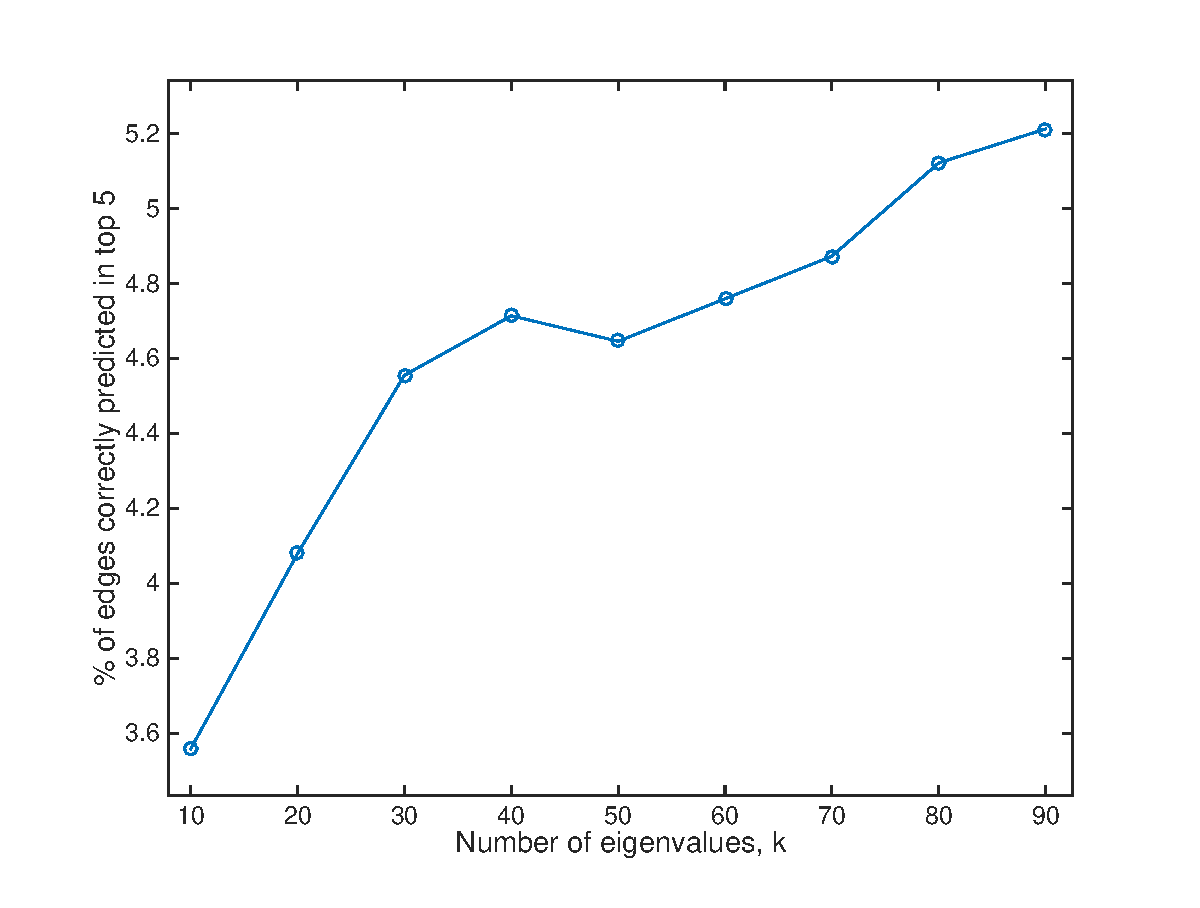
\includegraphics[width=\textwidth]{fb_eig_top5}
		\caption{Percentage of removed edges that have their end vertex in the top
    5 similar vertices of their start vertex, using $\bpos()$.}
    \label{fig:fb_eig_top5}
  \end{subfigure}%
  ~
  \begin{subfigure}[b]{0.5\textwidth}
    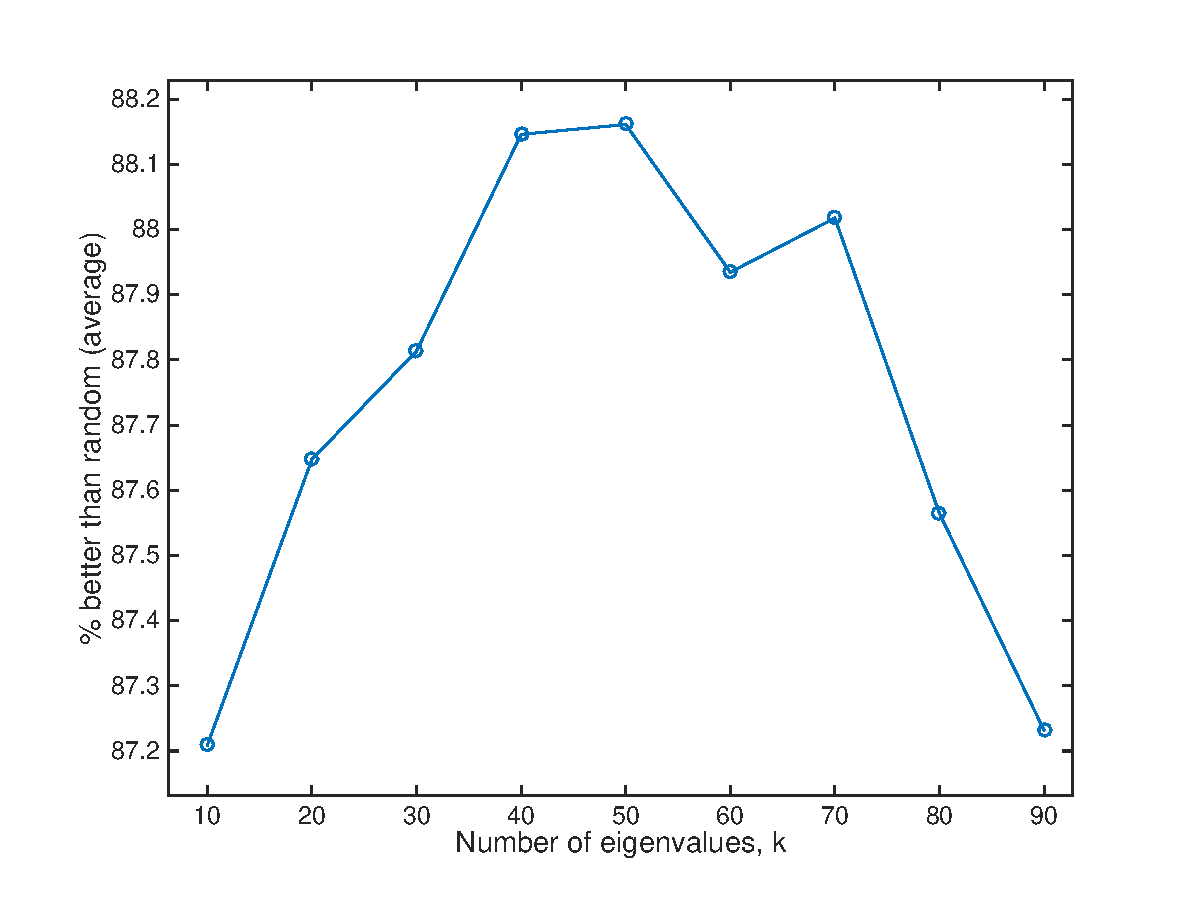
\includegraphics[width=\textwidth]{fb_eig_better}
		\caption{Percentage of test pairs that have a higher similarity
    than a random pair of vertices (that is not blacklisted).}
    \label{fig:fb_eig_better}
  \end{subfigure}
  \begin{subfigure}[b]{0.5\textwidth}
    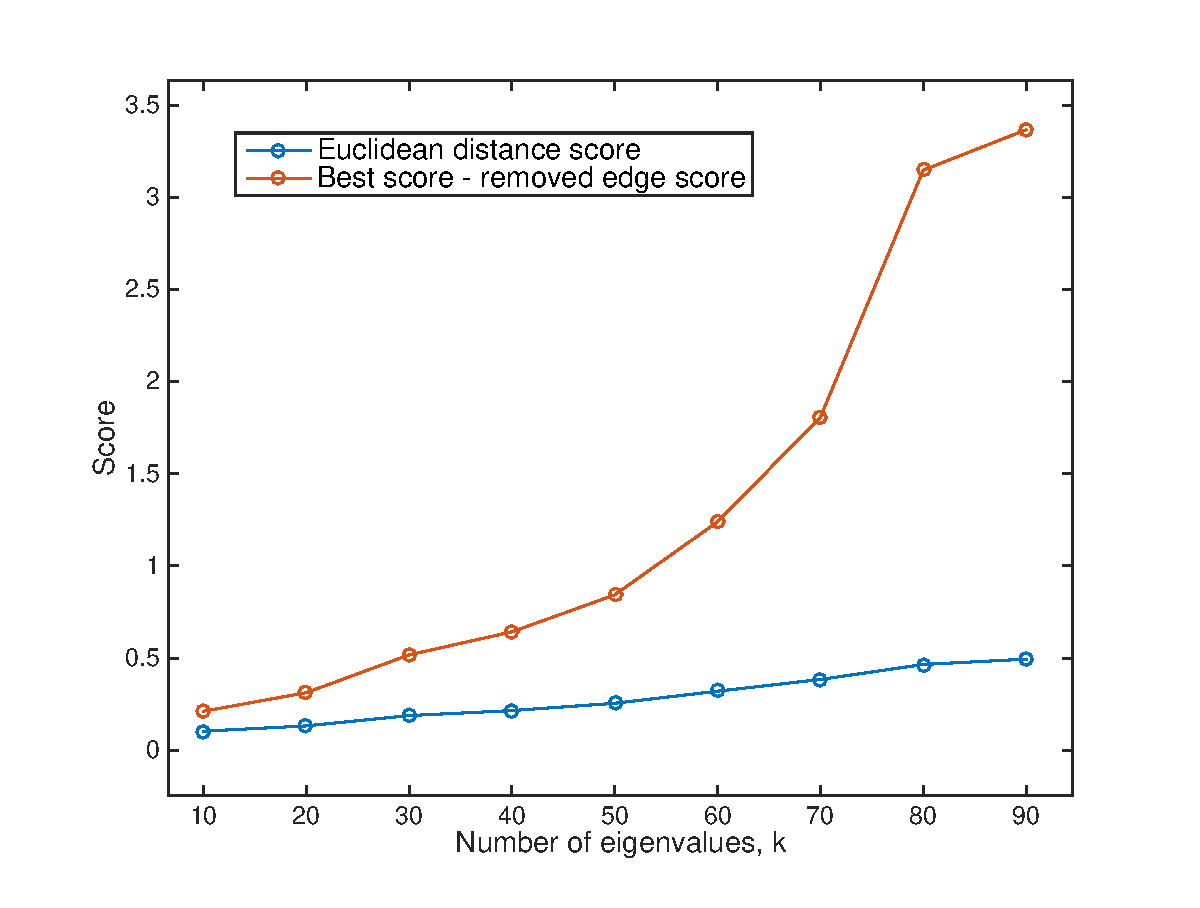
\includegraphics[width=\textwidth]{fb_eig_scores}
		\caption{Test pair and relative scores. $\mu = 0.5$.}
    \label{fig:fb_eig_scores}
  \end{subfigure}%
  ~
  \begin{subfigure}[b]{0.5\textwidth}
    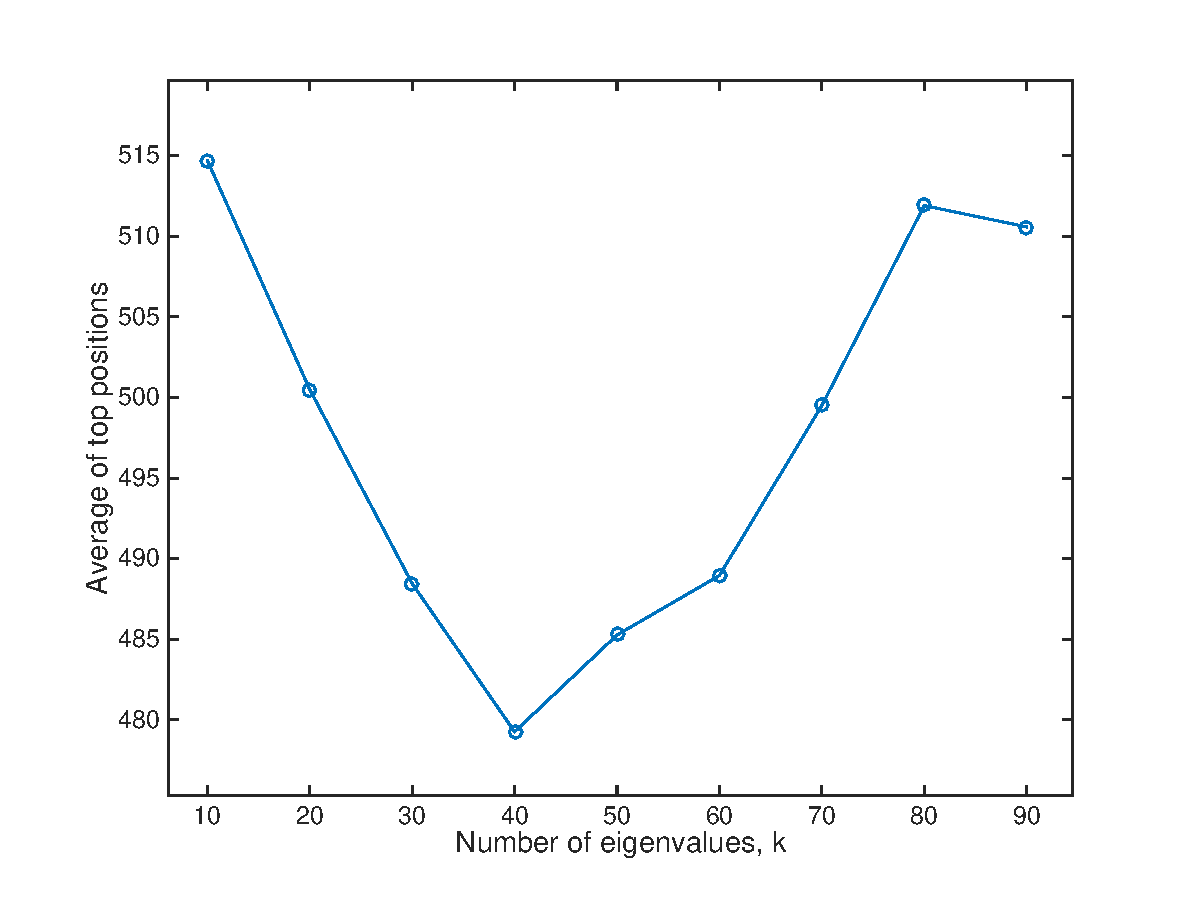
\includegraphics[width=\textwidth]{fb_eig_pos}
    \caption{Average sum of top positions.}
    \label{fig:fb_eig_pos}
  \end{subfigure}
  \caption{Different evaluation metrics on the friends dataset using the
  squared Euclidean distance between cloud vectors as the similarity measure
  (score).}
  \label{fig:fb_eval_euclidean}
\end{figure}

For a choice of $k=40$ and $\mu=0.5$, the algorithm performs between $88\%$ and
$88.5\%$ better than random at finding the randomly removed friendships. However,
the percentage of the removed edges that have a position in top 5 is arguably
low at around $4.6\%$; the percentage increases to around $15\%$ for top 20, and
to around $26\%$ for top 40 (1\% of the test set). It might be the case that
there are natural friendships in the dataset which are missing from the data. As
a conclusion, it can be argued that the algorithm performs reasonably well under
the assumption that the likelihood of two people being friends increases with
their network of common friends, but in reality the friendship relationship is
more complicated and depends on many features that are not modelled in this
dataset and not considered by this algorithm.



%
\subsection{Visualisation}
%\addcontentsline{toc}{subsection}{Visualisation}
%
A subjective method of evaluation is attempting to visualise the algorithm
output on real data and deduce whether it gives sensitive results. This method
has the disadvantage of being subjective and it cannot scale to very large
graphs, but it might give a broad idea of what the results are and help
fine-tune the algorithm on specific problems.

The undirected graph from \emph{Figure~\ref{fig:ci_diffusion}} was rendered
using Graphviz \cite{graphviz} in \emph{Figure~\ref{fig:visual_first}}, where the grey edges
represent real edges in the graph and the red edges represent similar vertices.
Only the top two similar vertices (that are not in Blacklist) are rendered. The
parameters used for the algorithm are $k=6$ and $\mu=0.5$. The graph has $31$
vertices and $41$ undirected edges.

\begin{figure}[tbp]
  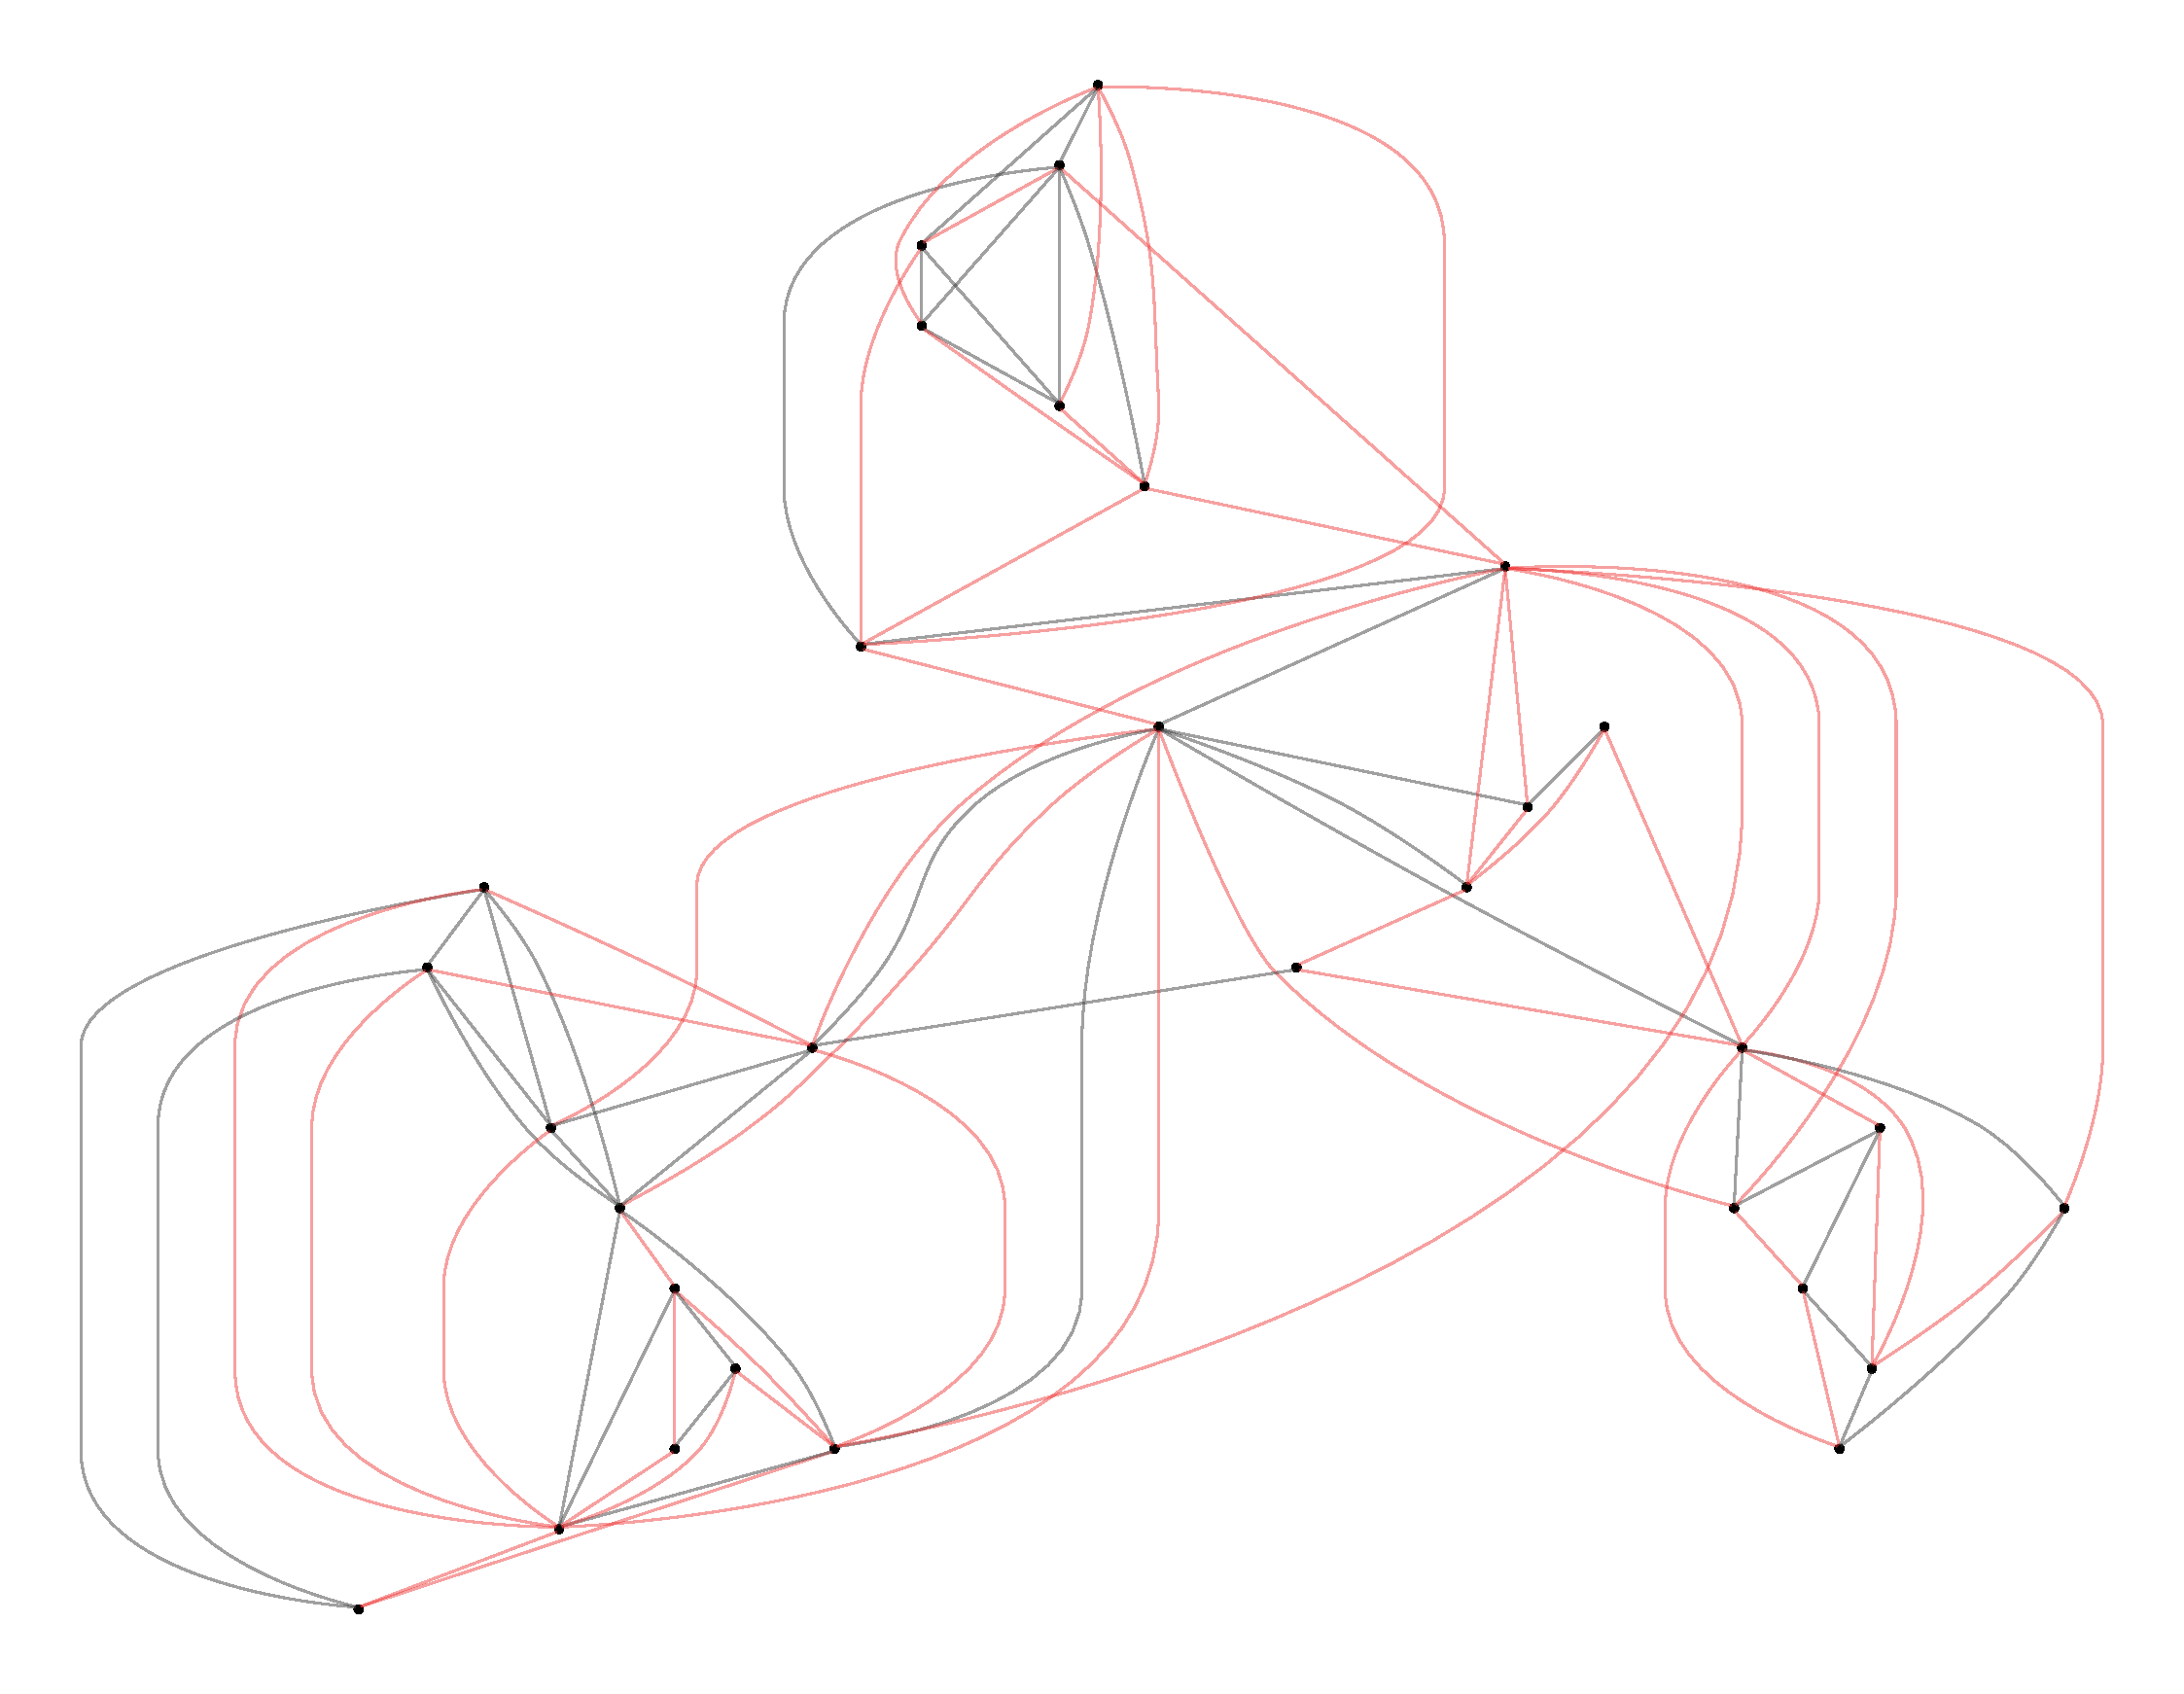
\includegraphics[width=\textwidth]{visual_first}
  \caption{Top 2 similar vertices on a small undirected graph. Grey edges are
  real edges in the graph and red edges represent similarities (top two of one
  of the vertices).}
  \label{fig:visual_first}
\end{figure}

The SNAP Facebook dataset with the top 5 similar vertices and parameters $k=40$
and $\mu=0.5$ is rendered in a similar way in \emph{Figure~\ref{fig:snap}}.

\begin{figure}[tbp]
  \includegraphics[width=\textwidth]{snap_big}
  \caption{SNAP Facebook dataset where the grey edges represent real friendships
  in the graph and the red edges represent similar vertices (in top 5 for each
  vertex).}
  \label{fig:snap}
\end{figure}


It is difficult to come to any conclusion based on the visualisation of the
results, especially on the larger graphs. However, having a way to visualise
the results can be helpful in some cases, especially for small graphs where
natural similarities are trivial to infer for the human eye.

%
%-------------------------------------------------------------------------------
% LIMITATIONS
%-------------------------------------------------------------------------------
%
\section{Limitations and future plans}
%
The current implementation of this algorithm has various limitations which are
discussed along with possible improvements.

The algorithm has only been evaluated on an undirected dataset of (arguably)
medium size. The next immediate step is to find directed graphs on which the
algorithm can be evaluated, and perform a similar evaluation. For larger graphs,
the evaluation process used so far would not scale and different, more efficient
methods will be required.

A comparison with similar algorithms, like the one described in
\cite{fouss2007random}, could be performed to see if this algorithm has
advantages compared to other work.

Cosine similarity and Euclidean distance similarity were presented in this report,
however only euclidean distance is well developed and evaluated. It is a trivial
task to add support for the cosine similarity, and then perform a similar
evaluation. After this, a comparison of the two metrics can be done.

In the real world datasets might have different types of relationships between
entities. Some relationship types might be more relevant than others in finding
a specific result. For instance, in a social network two people being friends
might be more relevant for recommending new friends than two people following the
same topic, but also using both features might be better than only one of them.
The current implementation of the algorithm can compute similarities if it is
given a weighted adjacency matrix but it does not have a way to automatically
obtain (learn) these weights from the dataset.


What if the dataset is too large to fit into main memory? The algorithm is
currently designed to run only on one machine, but finding ways to distribute it
over multiple machines will help run it on even larger datasets. One extension
of the algorithm is to make it suitable for distributed computing. An immediate
step could be distributing the computations of similarities and not the training,
because it reduces to simply distributing the storage of a matrix or two and
computing the dot product between two vectors or two vectors and a matrix.


Finding communities in graphs is not in the immediate goals of
this work but it can be extended to perform such tasks.
Instead of computing similarities between vertices directly, it might be useful
to try to apply different methods of clustering on the results to find a structure
of the graph.


The implementation for directed graphs has the limitation of needing to check
whether the eigenvalues are real or, if they are complex it needs to check if
the complex conjugate has also been computed. If these conditions aren't met for
an eigenpair, the whole eigenpair is dropped. A (small) optimisation could be to
find a way to compute the correct number of eigenpairs taking into consideration
the possibility of values being complex.

\newpage
\addcontentsline{toc}{section}{Bibliography}
\bibliography{ref.bib}{}
\bibliographystyle{plain}
\end{document}
